\section{The Least Squares (LS) Method}
\begin{itemize}
    \item The Least Squares (LS) estimator of the deterministic vector \(\theta\) search for the value of \(\theta\) which minimizes the \textit{distance} between the observed data vector and the SOI vector model,i.e. the values that provide the best match between the observed data and the model:
    \begin{align*}
\mathbf{x} = \mathbf{s}(\boldsymbol{\theta}) + \mathbf{e}
&\implies
\ \hat{\boldsymbol{\theta}}_{LS} = \arg\min_{\boldsymbol{\theta}} \|\mathbf{e}\|^2 = \arg\min_{\boldsymbol{\theta}} \sum_{i=0}^{N-1} e_i^2 \\[2ex]
\hat{\boldsymbol{\theta}}_{LS}
&= \arg\min_{\boldsymbol{\theta}} \| \mathbf{x} - \mathbf{s}(\boldsymbol{\theta}) \|^2 = \arg\min_{\boldsymbol{\theta}} \sum_{i=0}^{N-1} (x_i - s_i(\boldsymbol{\theta}))^2
\end{align*}

    \item \textbf{LS estimation} requires only knowledge of the signal model \(\mathbf{s}(\theta)\).
    \item if the signal vector depends linearly on the unknown parameters, then we call it \textbf{Linear Least Squares (LS)} estimator; if the dependency is not linear we call it \textbf{Non-Linear Least Squares (NLLS)} estimator.
    \item For example, in the case of a \textbf{sinusoid in noise}, the signal vector is a linear function only of the parameter \(A\), but it is a nonlinear function of \(\theta\) and \(F_0\):
\[
\mathbf{s}(\theta) \triangleq A \cdot \mathbf{p}(\theta, F_0)
= \frac{A}{\sqrt{2B}} \left[
\cos(\theta) \quad
\cos(2\pi F_0 + \theta) \quad
\cdots \quad
\cos\left( 2\pi F_0 \cdot (N-1) + \theta \right)
\right]^T
\]
    \item As we will see in the following, in the \textbf{linear} case, the \textbf{LS estimator} is much easier to derive, it can always be expressed \underline{in closed form}, and it is a linear function of the data.

\end{itemize}
\subsection{Solving linear equations}
\begin{itemize}
    \item Assume we have to solve a system of \(N\) linear equations with \(L\) unknowns:
    \begin{align*}
    \sum_{i=1}^L a_{ki} x_i = b_k, \qquad k = 1,2,\ldots,N
\end{align*}

\[
\begin{bmatrix}
a_{11} & a_{12} & \cdots & a_{1L} \\
a_{21} & a_{22} & \cdots & a_{2L} \\
a_{31} & a_{32} & \cdots & a_{3L} \\
\vdots & \vdots & \ddots & \vdots \\
a_{N1} & a_{N2} & \cdots & a_{NL}
\end{bmatrix}
\begin{bmatrix}
x_1 \\
x_2 \\
x_3 \\
\vdots \\
x_L
\end{bmatrix}
=
\begin{bmatrix}
b_1 \\
b_2 \\
b_3 \\
\vdots \\
b_N
\end{bmatrix}
\qquad
\rightarrow
\qquad
\mathbf{A}_{N \times L} \, \mathbf{x}_{L \times 1} = \mathbf{b}_{N \times 1}
\]
\textbf{Problem}: Given $\mathbf{A}$ and $\mathbf{b}$, determine $\mathbf{x}$.
\[
N~\text{number of equations}, \qquad L~\text{number of unknowns}
\]

\begin{align*}
N > L &\implies \text{overdetermined system (A is a ``tall matrix'')} \\
N < L &\implies \text{underdetermined system (A is a ``fat matrix'')}
\end{align*}
    \item if \(N<L\) there are more unknowns than equations, the linear system has \(\infty^{L-N}\) solutions.
    \item  if \(N=L\) the number of equations is equal to the number of unknowns in this case, if \textbf{A} is full rank, i.e. rank(\textbf{A})=\(N\), the system has only 1 solutions: \(\mathbf{x}=\mathbf{A}^{-1}\mathbf{b}\).
    \item if \(N>L\) there are more equations than unknowns. In this case, if \textbf{A} is full rank, i.e. rank(\textbf{A})=\(L\), the system has a solution only if the vector \textbf{b} belongs to the \(L\)-dim subspace generated by the \(L\) columns of \textbf{A}:
    \begin{align*}
\mathbf{A}_{N\times L} \; \mathbf{x}_{L\times 1} = \mathbf{b}_{N \times 1}
\qquad
\sum_{i=1}^L \mathbf{a}_i x_i = \mathbf{b}
\end{align*}

\[
\text{where} \quad \mathbf{A} =
\left[ \mathbf{a}_1 \quad \mathbf{a}_2 \quad \cdots \quad \mathbf{a}_L \right]
\]
\end{itemize}
\subsection{Linear Least Squares (LS)}
\begin{itemize}
    \item Aim of the \textbf{Least Squares (LS)} solution:
\begin{align*}
\text{Let us define:} \quad
\mathbf{e}_{N \times 1} \triangleq \mathbf{b}_{N \times 1} - \mathbf{A}_{N \times L} \mathbf{x}_{L \times 1}
\qquad\rightarrow\qquad
\mathbf{b} = \mathbf{A}\mathbf{x} + \mathbf{e},\ \text{where } N > L
\end{align*}
\vspace{-1em}
\[
\mathbf{e} \equiv \text{modeling error/measurement error}
\]
\vspace{-1em}
\begin{align*}
\mathbf{e} = [e_1 \quad e_2 \quad \cdots \quad e_N]^T
\qquad
\text{Error Energy:}\quad
E_e \triangleq \|\mathbf{e}\|^2 = \mathbf{e}^H\mathbf{e} = \sum_{i=1}^N |e_i|^2
\end{align*}

\[
\textbf{Problem:} \quad \text{find } \mathbf{x}\ \text{so that to minimize the energy of the error}\ \|\mathbf{e}\|^2
\]
    \item \textbf{Example}: let us consider an object that is moving of \underline{uniform rectilinear motion}. Its position at time \(t\) is given by \(p(t)=\alpha+\beta t\), with \(\alpha\) and \(\beta\) unknown parameters (\(\alpha\) is the initial position and \(\beta\) the speed).
    \item To estimate the two unknowns parameters, we can make two measurements of the object position at two different times. Obviously, the measurements will be affected by noise (e.g. internal noise of the measuring device):
    \begin{align*}
b(t) = p(t) + e(t) = \alpha + \beta t + e(t)
\end{align*}

\begin{align*}
\mathbf{b} =
\begin{bmatrix}
b(t_1) \\
b(t_2)
\end{bmatrix}
=
\begin{bmatrix}
\alpha + \beta t_1 + e(t_1) \\
\alpha + \beta t_2 + e(t_2)
\end{bmatrix}
=
\begin{bmatrix}
1 & t_1 \\
1 & t_2
\end{bmatrix}
\begin{bmatrix}
\alpha \\
\beta
\end{bmatrix}
+
\begin{bmatrix}
e(t_1) \\
e(t_2)
\end{bmatrix}
= \mathbf{A}\mathbf{x} + \mathbf{e}
\end{align*}

    \item Matrix \textbf{A} is known: it is determined by the kind of motion we hypothesize.
    \item If we solve the system of \(N=2\) linear equations in \(L=2\) unknowns, we obtain the parameters of the straight line that passes through the two positions we have measured:
\begin{figure}[H]
    \centering
    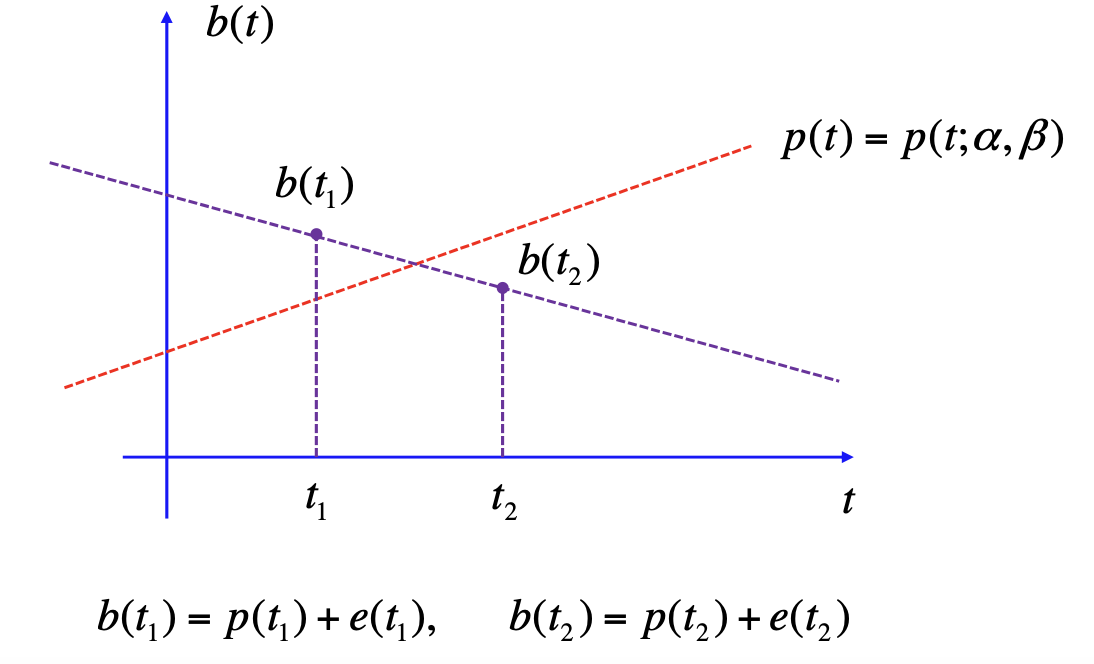
\includegraphics[width=0.55\linewidth]{Image/pdf 5/1.Two_equations.png}
    \label{fig:placeholder}
\end{figure}
    \item To reduce (i.e. average out) the effect of the measurement noise, we should collect \(N>2\) measurements:
    \begin{figure}[H]
        \centering
        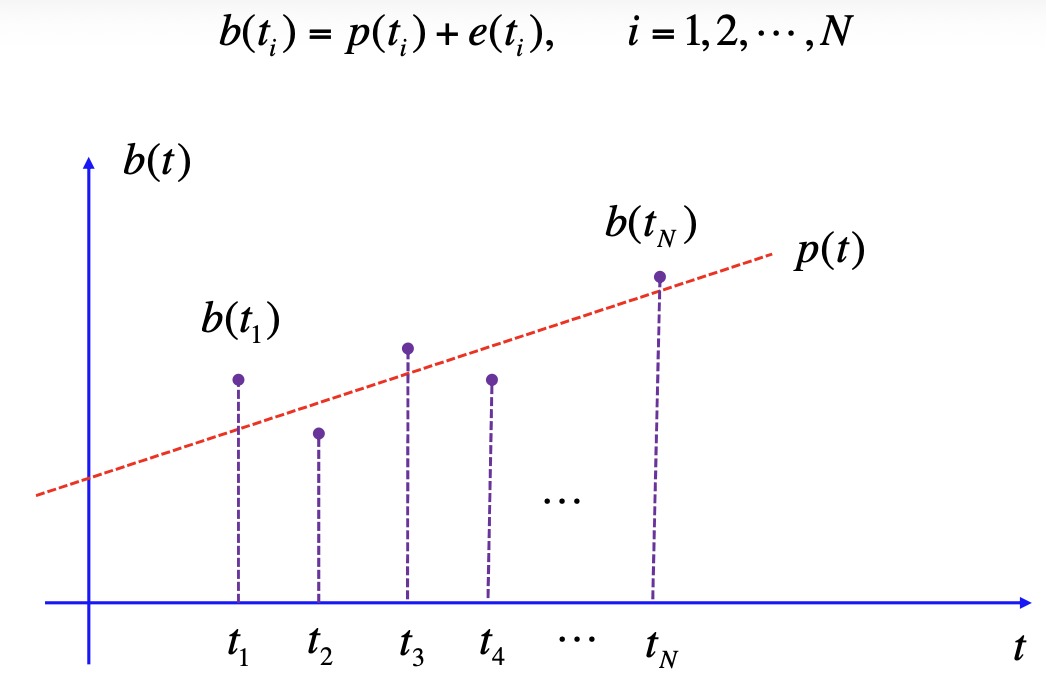
\includegraphics[width=0.6\linewidth]{Image/pdf 5/2.too_equations.png}
        \label{fig:placeholder}
    \end{figure}
    \item \(N\) measurements \(\rightarrow\) \(N\) equantion and \(L=2\) unknowns.
    \item It does not exists a solution to this linear overdetermined system of equations, i.e. it does not exists a straight line that passes through all the \(N\) points.
    \item The idea of the \textbf{\underline{Least Squares (LS)}} approach is to find the straight line that minimizes the energy of the errors betweem the measurements and the model (in this case: straight line motion). In other words, we look for the values of \(\alpha\) and \(\eta\) that minimizes the distance between model and measurements.
    \begin{figure}[H]
        \centering
        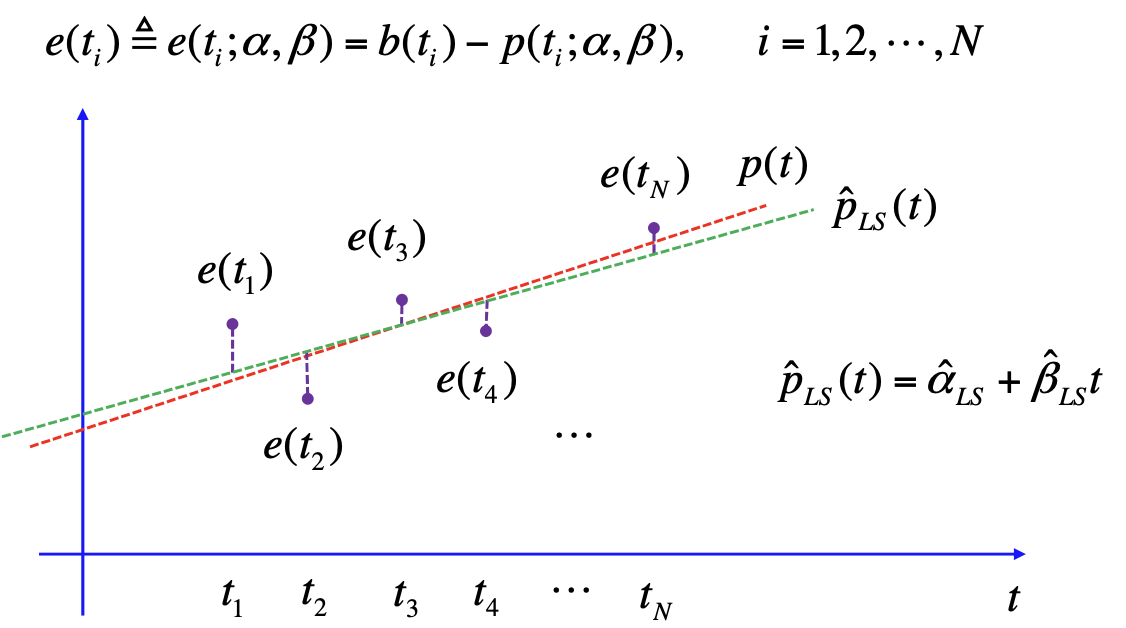
\includegraphics[width=0.55\linewidth]{Image/pdf 5/3.Approx.png}
        \label{fig:placeholder}
    \end{figure}
    \item The idea of the \textbf{\underline{Least Squares (LS)}} approach is to find the straight line that minimizes the energy of the errors between the measurements and the model:
\begin{align*}
\mathbf{b} =
\begin{bmatrix}
b(t_1) \\
b(t_2) \\
\vdots \\
b(t_N)
\end{bmatrix}
=
\begin{bmatrix}
1 & t_1 \\
1 & t_2 \\
\vdots & \vdots \\
1 & t_N
\end{bmatrix}
\begin{bmatrix}
\alpha \\
\beta
\end{bmatrix}
+
\begin{bmatrix}
e(t_1) \\
e(t_2) \\
\vdots \\
e(t_N)
\end{bmatrix}
= \mathbf{A}\mathbf{x} + \mathbf{e}
\end{align*}

\begin{align*}
\hat{\mathbf{x}}_{LS} = \arg\min_{\mathbf{x}} \| \mathbf{e} \|^2 = \arg\min_{\mathbf{x}} \| \mathbf{A}\mathbf{x} - \mathbf{b} \|^2
\end{align*}
\item Sta roba non viene chiesta si riporta per lo sport:
\begin{align*}
\|\mathbf{e}\|^2 = \mathbf{e}^H\mathbf{e} = \sum_{i=1}^N |e_i|^2 = \sum_{i=1}^N |e(t_i)|^2
\end{align*}
\begin{align*}
\|\mathbf{e}\|^2 &= \mathbf{e}^H \mathbf{e} = (\mathbf{A}\mathbf{x} - \mathbf{b})^H (\mathbf{A}\mathbf{x} - \mathbf{b}) 
= \mathbf{x}^H \mathbf{A}^H \mathbf{A} \mathbf{x} - \mathbf{b}^H \mathbf{A} \mathbf{x} - \mathbf{x}^H \mathbf{A}^H \mathbf{b} + \mathbf{b}^H \mathbf{b} \\
&= \mathbf{x}^H (\mathbf{A}^H \mathbf{A}) \mathbf{x} - \mathbf{b}^H \mathbf{A} (\mathbf{A}^H \mathbf{A})^{-1} (\mathbf{A}^H \mathbf{A}) \mathbf{x} 
- \mathbf{x}^H (\mathbf{A}^H \mathbf{A}) (\mathbf{A}^H \mathbf{A})^{-1} \mathbf{A}^H \mathbf{b} + \mathbf{b}^H \mathbf{b} \\
&= \left[\mathbf{x} - (\mathbf{A}^H \mathbf{A})^{-1} \mathbf{A}^H \mathbf{b}\right]^H (\mathbf{A}^H \mathbf{A}) \left[\mathbf{x} - (\mathbf{A}^H \mathbf{A})^{-1} \mathbf{A}^H \mathbf{b}\right] + \mathbf{b}^H \mathbf{b} \\
&\qquad - \mathbf{b}^H \mathbf{A} (\mathbf{A}^H \mathbf{A})^{-1} (\mathbf{A}^H \mathbf{A}) (\mathbf{A}^H \mathbf{A})^{-1} \mathbf{A}^H \mathbf{b} \\
&= \left[\mathbf{x} - (\mathbf{A}^H \mathbf{A})^{-1} \mathbf{A}^H \mathbf{b}\right]^H (\mathbf{A}^H \mathbf{A}) \left[\mathbf{x} - (\mathbf{A}^H \mathbf{A})^{-1} \mathbf{A}^H \mathbf{b}\right] + \mathbf{b}^H \mathbf{b}  \mathbf{b}^H \mathbf{A} (\mathbf{A}^H \mathbf{A})^{-1} \mathbf{A}^H \mathbf{b}\quad\\
&\text{[ we assume here that $\mathbf{A}$ is full rank ]}
\end{align*}
\begin{align*}
\|\mathbf{e}\|^2
    &= \left[\mathbf{x} - (\mathbf{A}^H \mathbf{A})^{-1} \mathbf{A}^H \mathbf{b}\right]^H (\mathbf{A}^H \mathbf{A}) \left[\mathbf{x} - (\mathbf{A}^H \mathbf{A})^{-1} \mathbf{A}^H \mathbf{b}\right] \\
    &\quad + \mathbf{b}^H \mathbf{b} - \mathbf{b}^H \mathbf{A} (\mathbf{A}^H \mathbf{A})^{-1} \mathbf{A}^H \mathbf{b} \\[2ex]
    &= \left[\mathbf{x} - \mathbf{A}^\# \mathbf{b}\right]^H (\mathbf{A}^H \mathbf{A}) \left[\mathbf{x} - \mathbf{A}^\# \mathbf{b}\right]
    + \mathbf{b}^H \left( \mathbf{I} - \mathbf{A} \mathbf{A}^\# \right) \mathbf{b}
\end{align*}
    \item The \(1^{st}\) term is always \(\geq\)0, whereas the \(2^{nd}\) term does not depend on \(\mathbf{x}\). Hence, the energy of the error is minimized when the \(1^{st}\) term is 0:
\[
\hat{\mathbf{x}}_{LS} = \mathbf{A}^{\#} \mathbf{b} = \left( \mathbf{A}^{H} \mathbf{A} \right)^{-1} \mathbf{A}^{H} \mathbf{b}
\qquad \text{Least Squares (LS) solution}
\]

\[
\mathbf{A}^{\#} \triangleq \left( \mathbf{A}^{H} \mathbf{A} \right)^{-1} \mathbf{A}^{H}
\qquad
{\color{blue} \text{Moore-Penrose pseudoinverse}}
\qquad \rightarrow \qquad
\mathbf{A}^{\#}_{L\times N}\;
\mathbf{A}_{N\times L} = \mathbf{I}_{L\times L}
\]

    \item Geometric interpretation of the \textbf{linear Least Squares (LS)} solution:
\begin{figure}[H]
    \centering
    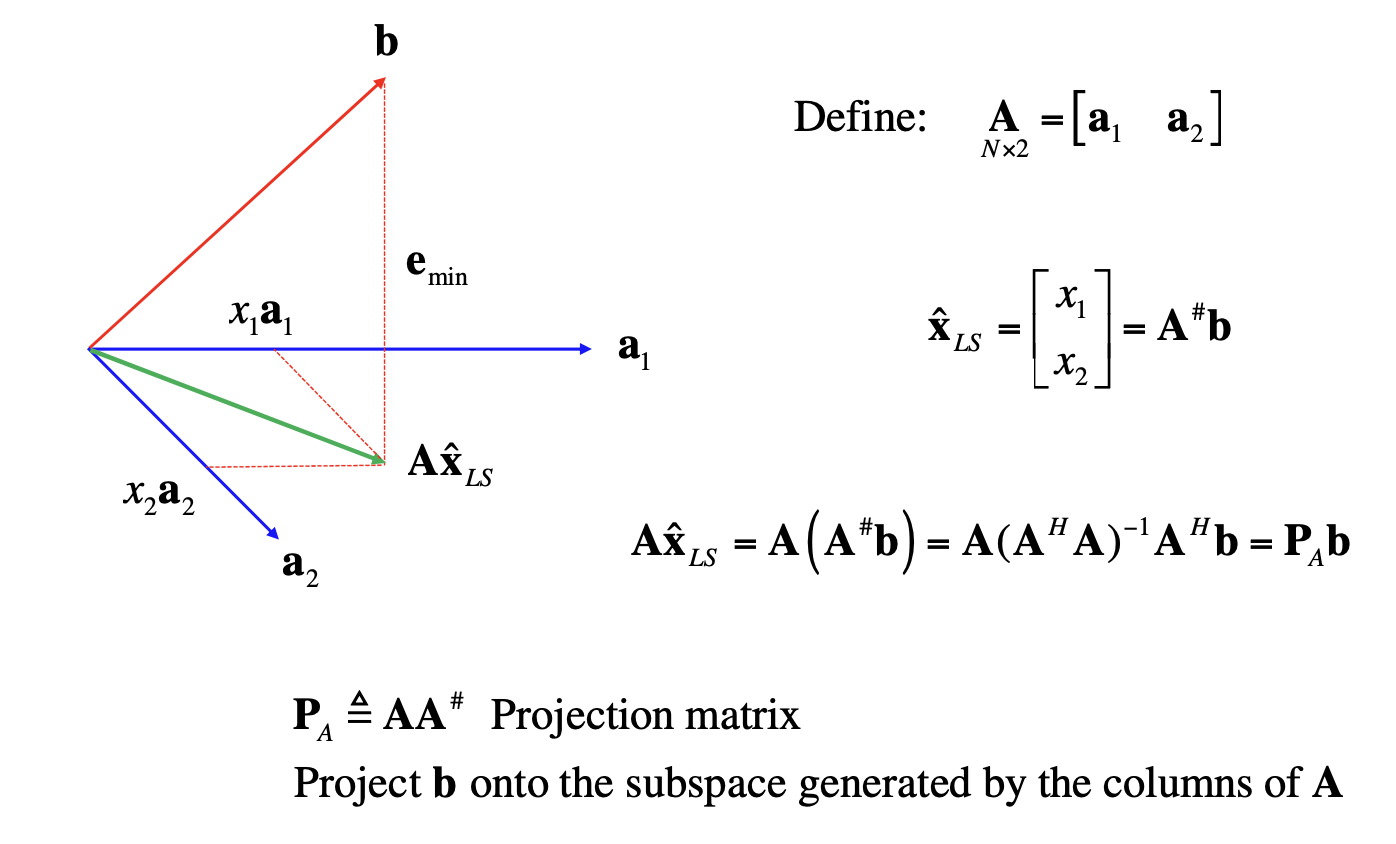
\includegraphics[width=0.6\linewidth]{Image/pdf 5/4.Geom_rapp.png}
    \label{fig:placeholder}
\end{figure}
\item Some important properties: \(\mathbf{P}_A\triangleq \mathbf{AA}^\#\)
\begin{itemize}
    \item Property 1: \(\mathbf{P}_A=\mathbf{P_A}^2\) (Idempotent)
    \item Property 2: \(\mathbf{P}_A=\mathbf{P}_A^H\) (Hermitian)
\end{itemize}
\item Other Formulas
\[
\mathbf{\hat{x}}_{LS}=\begin{bmatrix}
    x_1 \\x_2
\end{bmatrix}=\mathbf{A}^{\#}\mathbf{b}
\]
\[
\underline{\mathbf{e}}_{\min} = \mathbf{b} - \mathbf{A} \hat{\mathbf{x}}_{LS}
= \mathbf{b} - \mathbf{P}_A \mathbf{b}
= \left(\mathbf{I} - \mathbf{P}_A\right)\mathbf{b}
= \mathbf{P}_A^{\perp} \mathbf{b}
\]
\[
\mathbf{P}_A^{\perp} = \text{Projection matrix onto the subspace} \\
\quad{\perp}\;\; \text{the columns of}\;\;\mathbf{A}
\]
\[
\mathbf{P}_A{}_{N \times N} 
= \mathbf{A}_{N \times L} \, \mathbf{A}^{\#}_{L \times N}
\qquad \neq \qquad
\mathbf{A}^{\#}_{L \times N} \, \mathbf{A}_{N \times L}
= \mathbf{I}_{L \times L}
\]
\begin{align*}
\left\| \mathbf{e}_{\min} \right\|^2 
&= \mathbf{e}_{\min}^{H} \mathbf{e}_{\min} = \left( \mathbf{P}_A^{\perp} \mathbf{b} \right)^{H} \mathbf{P}_A^{\perp} \mathbf{b} = \mathbf{b}^{H} \left( \mathbf{P}_A^{\perp} \right)^{H} \mathbf{P}_A^{\perp} \mathbf{b} \\
&= \mathbf{b}^{H} \mathbf{P}_A^{\perp} \mathbf{P}_A^{\perp} \mathbf{b} = \mathbf{b}^{H} \mathbf{P}_A^{\perp} \mathbf{b} = \mathbf{b}^{H} \left( \mathbf{I} - \mathbf{A} \mathbf{A}^{\#} \right) \mathbf{b}
\end{align*}
\item The linear LS solution is the vector \textbf{x} that makes the error \textbf{e} orthogonal to the range of \textbf{A}, i.e. the subspace spanned by the columns of \textbf{A}: \textbf{Orthogonality Principle}(a.k.a \textbf{Projection Theorem}).

\end{itemize}
\subsubsection{EigenValue Decomposition (EVD)}
\begin{itemize}
    \item \textbf{EigenValue Decomposition (EVD)} of an \underline{Hermitian square} matrix:
\begin{align*}
\mathbf{A}_{N \times N} 
&= \mathbf{U}_{N \times N} \; \mathbf{\Lambda}_{N \times N} \; \mathbf{U}^{H}_{N \times N}
= \sum_{i=1}^{N} \lambda_i \mathbf{u}_i \mathbf{u}_i^{H}
\end{align*}

\[
\mathbf{U} = [\mathbf{u}_1 \;\; \mathbf{u}_2 \;\; \cdots \;\; \mathbf{u}_N], \quad 
\text{unitary matrix of the eigenvectors}
\qquad
\mathbf{U}^{-1} = \mathbf{U}^{H}
\]

\[
\mathbf{\Lambda}
= \begin{bmatrix}
\lambda_1 & 0 & \cdots & 0 \\
0 & \lambda_2 & \cdots & 0 \\
\vdots & \vdots & \ddots & \vdots \\
0 & 0 & \cdots & \lambda_N
\end{bmatrix},
\quad
\text{diagonal matrix of the eigenvalues (all real)}
\]
    \item if \textbf{A} is full rank, i.e. all \(\lambda_i\neq0\), then we can calculate the inverse of \textbf{A} as:
    \[
\mathbf{A}^{-1}
= \left( \mathbf{U} \mathbf{\Lambda} \mathbf{U}^{H} \right)^{-1}
= \mathbf{U} \mathbf{\Lambda}^{-1} \mathbf{U}^{H}
\]
\end{itemize}
\subsubsection{Singular Value Decomposition (SVD)}
\begin{itemize}
    \item The \textbf{Singular Value Decomposition (SVD)} is a generalization of the EVD for rectangular matrices:
\begin{align*}
\mathbf{A}_{N \times L}
&= \mathbf{U}_{N \times N} \; \mathbf{\Sigma}_{N \times L} \; \mathbf{V}^{H}_{L \times L}
= \sum_{i=1}^{L} \sigma_i \mathbf{u}_i \mathbf{v}_i^{H}
\end{align*}

\[
\mathbf{U} = [\mathbf{u}_1 ~ \mathbf{u}_2 ~ \cdots ~ \mathbf{u}_N],
\quad \text{unitary matrix of the left singular vectors}
\]

\[
\mathbf{V} = [\mathbf{v}_1 ~ \mathbf{v}_2 ~ \cdots ~ \mathbf{v}_L],
\quad \text{unitary matrix of the right singular vectors}
\]

\[
\mathbf{\Sigma} =
\begin{bmatrix}
\sigma_1 & 0      & \cdots & 0      \\
0        & \sigma_2 & \cdots & 0      \\
\vdots   & \vdots & \ddots & \vdots \\
0        & 0      & \cdots & \sigma_L \\
0        & 0      & \cdots & 0 \\
\vdots   & \vdots &        & \vdots
\end{bmatrix},
\quad \text{matrix of the singular values (real, $\geq$ 0)}
\]

\[
\;\;\;\;\;\sigma_1 \geq \sigma_2 \geq \cdots \geq \sigma_L \geq 0
\]

\[
\textcolor{blue}{\blacksquare\;\; \text{Hypothesis:}~ N > L~ \text{(tall matrix)}}
\]

    \item If matrix \textbf{A} is not full-rank, for example: \textit{rank}(\textbf{A})=\(r<L\) then, we have :
\[
\sigma_1 \geq \sigma_2 \geq \cdots \geq \sigma_r > 0
\quad \text{and} \quad
\sigma_{r+1} = \sigma_{r+2} = \cdots = \sigma_L = 0
\]

\[
\mathbf{U} = \left[ \mathbf{U}_1 \;\; \mathbf{U}_2 \right], \quad
\text{where}
\quad
\mathbf{U}_1 = \left[ \mathbf{u}_1 \;\; \mathbf{u}_2 \;\; \cdots \;\; \mathbf{u}_r \right],\;\;
\mathbf{U}_2 = \left[ \mathbf{u}_{r+1} \;\; \cdots \;\; \mathbf{u}_N \right],
\]

\[
\mathbf{V} = \left[ \mathbf{V}_1 \;\; \mathbf{V}_2 \right], \quad
\text{where}
\quad
\mathbf{V}_1 = \left[ \mathbf{v}_1 \;\; \mathbf{v}_2 \;\; \cdots \;\; \mathbf{v}_r \right],\;\;
\mathbf{V}_2 = \left[ \mathbf{v}_{r+1} \;\; \cdots \;\; \mathbf{v}_L \right],
\]

\[
\mathbf{\Sigma} = 
\begin{bmatrix}
\mathbf{\Sigma}_1 & 0 \\
0 & 0
\end{bmatrix}, 
\quad \text{where} \quad
\mathbf{\Sigma}_1 = 
\begin{bmatrix}
\sigma_1 & 0 & \cdots & 0 \\
0 & \sigma_2 & \cdots & 0 \\
\vdots & \vdots & \ddots & \vdots \\
0 & 0 & \cdots & \sigma_r
\end{bmatrix}
\]
    \item Matrix \textbf{A} not full-rank: \textit{rank}(\textbf{A})=\(r<L\)
    \[
\mathbf{U} = [\mathbf{U}_1 ~ \mathbf{U}_2], \quad
\mathbf{V} = [\mathbf{V}_1 ~ \mathbf{V}_2], \quad
\mathbf{\Sigma} = 
\begin{bmatrix} 
\mathbf{\Sigma}_1 & 0 \\ 
0 & 0 
\end{bmatrix}
\]

\begin{align*}
\mathbf{A}_{N \times L} 
&= \mathbf{U}_{N \times N} \mathbf{\Sigma}_{N \times L} \mathbf{V}^{H}_{L \times L} \\[1em]
&= 
\begin{bmatrix}\mathbf{U}_1 & \mathbf{U}_2\end{bmatrix}
\begin{bmatrix}\mathbf{\Sigma}_1 & 0 \\ 0 & 0\end{bmatrix}
\begin{bmatrix}\mathbf{V}_1 & \mathbf{V}_2\end{bmatrix}^{H} \\[1em]
&= 
\begin{bmatrix}\mathbf{U}_1 & \mathbf{U}_2\end{bmatrix}
\begin{bmatrix}\mathbf{\Sigma}_1 & 0 \\ 0 & 0\end{bmatrix}
\begin{bmatrix}\mathbf{V}_1^{H} \\ \mathbf{V}_2^{H}\end{bmatrix} \\[1em]
&= 
\begin{bmatrix}\mathbf{U}_1 \mathbf{\Sigma}_1 & 0\end{bmatrix}
\begin{bmatrix}\mathbf{V}_1^{H} \\ \mathbf{V}_2^{H}\end{bmatrix} \\[1em]
&= \mathbf{U}_1 \mathbf{\Sigma}_1 \mathbf{V}_1^{H}{}_{N \times r ~ r \times r ~ r \times L}
\end{align*}
\[
\mathbf{A}_{N \times L}
= \mathbf{U}_{N \times N} \mathbf{\Sigma}_{N \times L} \mathbf{V}^{H}_{L \times L}
= \mathbf{U}_1{}_{N \times r} \;\mathbf{\Sigma}_1{}_{r \times r}\; \mathbf{V}_1^{H}{}_{r \times L}
\]
    \item Efficient calculation of the pseudoinverse of \textbf{A} is based on the SVD.
    \item Assume first that \textbf{A} is \underline{full rank}, i.e. \(r=\min(L,N)=L\):
    \[
\mathbf{A}_{N \times L}
= \mathbf{U}_1{}_{N \times L}
\mathbf{\Sigma}_1{}_{L \times L}
\mathbf{V}_1^{H}{}_{L \times L}
,\quad
\text{where } \mathbf{V}_1^{-1} = \mathbf{V}_1^{H}
\]
\vspace{-0.5em}
\begin{align*}
\mathbf{A}^{\#}_{L \times N}
&= (\mathbf{A}^{H}\mathbf{A})^{-1} \mathbf{A}^{H} = \left(\mathbf{V}_1 \mathbf{\Sigma}_1 \mathbf{U}_1^{H} \mathbf{U}_1 \mathbf{\Sigma}_1 \mathbf{V}_1^{H}\right)^{-1} \mathbf{V}_1 \mathbf{\Sigma}_1 \mathbf{U}_1^{H} \\
&= \left(\mathbf{V}_1 \mathbf{\Sigma}_1^2 \mathbf{V}_1^{H}\right)^{-1} \mathbf{V}_1 \mathbf{\Sigma}_1 \mathbf{U}_1^{H} = \mathbf{V}_1 \mathbf{\Sigma}_1^{-2} \mathbf{V}_1^{H} \mathbf{V}_1 \mathbf{\Sigma}_1 \mathbf{U}_1^{H}\\
&= \mathbf{V}_1 \mathbf{\Sigma}_1^{-1} \mathbf{U}_1^{H}
\end{align*}
\vspace{-0.5em}
\begin{align*}
\mathbf{A}^{\#} \mathbf{A}
&= \mathbf{V}_1 \mathbf{\Sigma}_1^{-1} \mathbf{U}_1^{H} \mathbf{U}_1 \mathbf{\Sigma}_1 \mathbf{V}_1^{H}= \mathbf{V}_1 \mathbf{V}_1^{H} = \mathbf{I}_{L\times L}
\end{align*}
\newpage
\item if \textbf{A} is not full rank, i.e. \(r<L\):
\[
\underset{N \times L}{\mathbf{A}}
=
\underset{N \times N}{\mathbf{U}}
\;\;
\underset{N \times L}{\mathbf{\Sigma}}
\;\;
\underset{L \times L}{\mathbf{V}^H}
=
\underset{N \times r}{\mathbf{U}_1}
\;\;
\underset{r \times r}{\mathbf{\Sigma}_1}
\;\;
\underset{r \times L}{\mathbf{V}_1^H}
\]

\[
\underset{L \times N}{\mathbf{A}^{\#}}
=
\left(
\underset{N \times N}{\mathbf{U}}
\;\;
\underset{N \times L}{\mathbf{\Sigma}}
\;\;
\underset{L \times L}{\mathbf{V}^H}
\right)^{\#}
=
\left(\mathbf{V}^H\right)^{\#}
\;
\Sigma^{\#}
\;
\mathbf{U}^{\#}
=
\mathbf{V} \Sigma^{\#} \mathbf{U}^H
=
\mathbf{V}_1 \Sigma_1^{-1} \mathbf{U}_1^H
\]

\[
\text{where:}
\]

\[
\boldsymbol{\Sigma} =
\begin{bmatrix}
\boldsymbol{\Sigma}_1 & 0 \\
0 & 0
\end{bmatrix}
\Longrightarrow
\boldsymbol{\Sigma}^{\#} \triangleq
\begin{bmatrix}
\boldsymbol{\Sigma}_1^{-1} & 0 \\
0 & 0
\end{bmatrix}
\Longrightarrow
\boldsymbol{\Sigma}^{\#}\boldsymbol{\Sigma} =
\begin{bmatrix}
\mathbf{I} & 0 \\
0 & 0
\end{bmatrix}
\]

\[
\underset{L \times N}{\mathbf{A}^{\#}}
\;
\underset{N \times L}{\mathbf{A}}
=
{\mathbf{V}_1 \Sigma_1^{-1} \mathbf{U}_1^H \mathbf{U}_1 \Sigma_1 \mathbf{V}_1^H}
=
{\mathbf{V}_1 \mathbf{V}_1^H}
\neq
\underset{L \times L}{\mathbf{I}}
\quad
\left(
\mathbf{V}_1^H \mathbf{V}_1 = \underset{r \times r}{\mathbf{I}}
\right)
\]
\item \textbf{IMPORTANT} if \textbf{A} is a square full-rank matrix: \(\mathbf{A}^{\#}=\mathbf{A}^{-1}\), if it is also Hermitian: \(\mathbf{V}=\mathbf{U}\)
\item If the \underline{square matrix} \textbf{A} is not Hermitian and some eigenvalues have geometric multiplicity (i.e. the number of linearly independent eigenvectors related to that eigenvalue) lower than its algebraic multiplicity (\(>1\)), the eigenvector cannot be inverted and matrix \textbf{A} cannot be factorized (diagonalized),as previously described:
\[
\boxed{
    \mathbf{A}\mathbf{U} = \mathbf{U}\boldsymbol{\Sigma}
    \quad \overset{\text{U full-rank}}{ \implies }
    \mathbf{A} = \mathbf{U}\boldsymbol{\Sigma}\mathbf{U}^{-1}
    \quad \overset{\text{A Hermitian}}{ \implies}
    \mathbf{A} = \mathbf{U}\boldsymbol{\Sigma}\mathbf{U}^H
}
\]

\[
\mathbf{A} = \begin{bmatrix} 1 & 1 \\ 0 & 1 \end{bmatrix}, 
\quad \textit{EVD}:\quad \mathbf{A}\mathbf{U} = \mathbf{U}\boldsymbol{\Sigma}
\implies
\mathbf{U} = \begin{bmatrix} 1 & -1 \\ 0 & 0 \end{bmatrix},\quad
\boldsymbol{\Sigma} = \begin{bmatrix} 1 & 0 \\ 0 & 1 \end{bmatrix}
\]

\[
\mathbf{A}^{-1} = \begin{bmatrix} 1 & -1 \\ 0 & 1 \end{bmatrix}
\]
\item \textbf{A} cannot be factorized as \(\mathbf{A=U}\boldsymbol{\Sigma}\mathbf{U}^{-1}\) since matrix \textbf{U} cannot be inverted, so we cannot derive the inverse of \textbf{A} as \(\mathbf{A^{-1}=U}\boldsymbol{\Sigma}^{-1}\mathbf{U}^{-1}\).

\item Instead, the SVD of the (square) matrix \textbf{A} exist and it is given by:
\[
\mathit{SVD}: \quad \mathbf{A} = \mathbf{U} \boldsymbol{\Sigma} \mathbf{V}^H
\implies
\mathbf{U} =
\begin{bmatrix}
0.8507 & -0.5257 \\
0.5257 & 0.8507
\end{bmatrix}
\]

\[
\boldsymbol{\Sigma} =
\begin{bmatrix}
1.618 & 0 \\
0 & 0.618
\end{bmatrix}
\qquad
\mathbf{V} =
\begin{bmatrix}
0.5257 & -0.8507 \\
0.8507 & 0.5257
\end{bmatrix}
\]

\[
\mathbf{A}^{\#} = \mathbf{V} \boldsymbol{\Sigma}^{-1} \mathbf{U}^H
=
\begin{bmatrix}
1 & -1 \\
0 & 1
\end{bmatrix}
= \mathbf{A}^{-1}
\]
\[
\text{SVD of } \mathbf{A} \text{ when } \operatorname{rank}(\mathbf{A}) = r,\ \text{with } r \leq L < N
\]

\[
\boxed{
\underset{N \times L}{\mathbf{A}}
=
\underset{N \times N}{\mathbf{U}}
\;\;
\underset{N \times L}{\mathbf{\Sigma}}
\;\;
\underset{L \times L}{\mathbf{V}^H}
=
\begin{bmatrix}
\mathbf{U}_1 & \mathbf{U}_2
\end{bmatrix}
\begin{bmatrix}
\mathbf{\Sigma}_1 & 0 \\
0 & 0
\end{bmatrix}
\begin{bmatrix}
\mathbf{V}_1^H \\
\mathbf{V}_2^H
\end{bmatrix}
=
\underset{N\times r}{\mathbf{U}_1}
\;
\underset{r\times r}{\mathbf{\Sigma}_1}
\;
\underset{r\times L}{\mathbf{V}_1^H}
}
\]
\[
\underset{L \times N}{\mathbf{A}^{\#}}
=
\underset{L\times r}{\mathbf{V}_1}
\;
\underset{r\times r}{\mathbf{\Sigma}_1^{-1}}
\;
\underset{r\times N}{\mathbf{U}_1^H}
\]
\item \underline{\textbf{Least Squares (LS)} solution of the overdetermined linear system:}
\[
\mathbf{b} = \mathbf{A}\mathbf{x} + \mathbf{e}
\]
\vspace{-1em}
\[
\textbf{Problem:}\quad \text{find } \mathbf{x} \text{ such that }
\|\mathbf{e}\|^2 = \|\mathbf{A}\mathbf{x} - \mathbf{b}\|^2 \text{ is minimum.}
\]

\[
\textbf{Solution:}\quad
\hat{\mathbf{x}}_{LS} = \mathbf{A}^{\#}\mathbf{b}, \quad \text{where} \quad
\underset{L\times N}{\mathbf{A}^{\#}}
=
(\mathbf{A}^H\mathbf{A})^{-1}\mathbf{A}^H
=
\mathbf{V}_1 \boldsymbol{\Sigma}_1^{-1} \mathbf{U}_1^H
\]
\end{itemize}
\subsection{The deterministic linear model}
\begin{itemize}
    \item When the \textbf{signal of interest (SOI)} can be expressed as a linear combination of \(p\) vector, \(\mathbf{h}_i\), i.e. \textbf{S} belongs to the linear subspace generated by the \(p\) vectors \(\mathbf{h}_i\), with \(p\leq N\), then we have:
    \[
\underset{N \times 1}{\mathbf{X}}
=
\mathbf{S} + \mathbf{W}
=
\underset{N \times p}{\mathbf{H}}
\underset{p \times 1}{\boldsymbol{\theta}}
+ \mathbf{W}
=
\sum_{i=1}^{p} \theta_i \mathbf{h}_i + \mathbf{W}
\]

\[
\underset{N \times p}{\mathbf{H}} \triangleq
\big[\, \mathbf{h}_1 \ \mathbf{h}_2 \ \cdots \ \mathbf{h}_p \,\big],
\qquad
\underset{p \times 1}{\boldsymbol{\theta}} \triangleq
\begin{bmatrix}
\theta_1 \\
\theta_2 \\
\vdots \\
\theta_p
\end{bmatrix}
\]
    \begin{itemize}
        \item \textbf{X} = observed data vector
        \item \textbf{W} = measurament error and/lr modeling error
        \item \(N\) = number of measurements (number of equations)
        \item \(p\) = number of unknowns
        \item \(N>p\)\quad\(\rightarrow\)\quad overdetermined system (\textbf{H} is a "full matrix")
    \end{itemize}
\end{itemize}
\subsubsection{Linear Least Squares (LS)}
\begin{itemize}
    \item \textbf{Problem}: Given the observed data vector \textbf{X} and given \textbf{H}, a priori known, derive an estimate of the deterministic unknown parameter vector \(\theta\).
    \item \textbf{Linear Least Squares (LS) estimate}:

    \item Note that once \(\theta\) has been estimated, we can estimate the signal as
    \[
    \mathbf{\hat{S}_{LS}} = \mathbf{H}\boldsymbol{\hat{\theta}_{LS}}
    \]
\end{itemize}
\subsubsection{LS vs ML estimation}
\begin{itemize}
    \item Let us go back to our problem of \underline{estimating the parameters of a deterministic real-valued signal}\\
    \underline{observed in the presence of AWGN}, given \(N\) samples of the received signal:
    \[
\mathbf{X} = \mathbf{s}(\boldsymbol{\theta}) + \mathbf{W}, 
\qquad
\mathbf{W} \in \mathcal{N}\big( \mathbf{0}, \mathbf{R} \big), 
\qquad
\mathbf{R} = E\left\{ \mathbf{W}\mathbf{W}^T \right\} 
= \sigma_W^{2}\,\mathbf{I}
\]
    \item \textbf{Problem}: Assuming that the relationship between the signal and the unknown parameters is \underline{known}, derive the \textbf{ML} estimator of \(\theta\).
\newpage
    \item \textbf{Assumption}: the real-valued noise is additive, white and Gaussian (AWGN), so the joint pdf is:
    \[
f_{\mathbf{X}}(\mathbf{x}; \boldsymbol{\theta})
=
\frac{1}{\sqrt{(2\pi)^{N} \, |\mathbf{R}|}}
\exp\!\left(
-\frac{1}{2}
\big(\mathbf{x} - \mathbf{s}(\boldsymbol{\theta})\big)^{T}
\mathbf{R}^{-1}
\big(\mathbf{x} - \mathbf{s}(\boldsymbol{\theta})\big)
\right)
\]

\[
|\mathbf{R}| = \det\{\mathbf{R}\},
\qquad
\mathbf{R} = \mathbf{R}^{T}
\quad\text{positive definite (so symmetric) matrix}
\]
\[
\mathbf{R} = \sigma_W^{2}\mathbf{I}
\quad \Longrightarrow \quad
f_{\mathbf{X}}(\mathbf{x}; \boldsymbol{\theta})
=
\frac{1}{\sqrt{(2\pi\sigma_W^{2})^{N}}}
\exp\!\left(
-\frac{1}{2\sigma_W^{2}}
\big(\mathbf{x} - \mathbf{s}(\boldsymbol{\theta})\big)^{T}
\big(\mathbf{x} - \mathbf{s}(\boldsymbol{\theta})\big)
\right)
\]

\[
\ln L(\boldsymbol{\theta})
=
\ln f_{\mathbf{X}}(\mathbf{x}; \boldsymbol{\theta})
=
\kappa
-\frac{1}{2\sigma_W^{2}}
\big(\mathbf{x} - \mathbf{s}(\boldsymbol{\theta})\big)^{T}
\big(\mathbf{x} - \mathbf{s}(\boldsymbol{\theta})\big)
\]

\[
=
\kappa
-\frac{1}{2\sigma_W^{2}}
\sum_{n=0}^{N-1}
\big(x_n - s_n(\boldsymbol{\theta})\big)^{2}
=
\kappa
-\frac{1}{2\sigma_W^{2}}
\left\|\mathbf{x} - \mathbf{s}(\boldsymbol{\theta})\right\|^{2}
\]

\[
\hat{\boldsymbol{\theta}}_{ML}
=
\arg\max_{\boldsymbol{\theta}} \ln L(\boldsymbol{\theta})
=
\arg\min_{\boldsymbol{\theta}}
\left\|\mathbf{x} - \mathbf{s}(\boldsymbol{\theta})\right\|^{2}
=
\hat{\boldsymbol{\theta}}_{LS}
\]
\[
\text{AWGN}
\quad \Longrightarrow \quad
\hat{\boldsymbol{\theta}}_{ML}
=
\arg\max_{\boldsymbol{\theta}} \ln f_{\mathbf{X}}(\mathbf{x}; \boldsymbol{\theta})
=
\arg\min_{\boldsymbol{\theta}}
\left\| \mathbf{x} - \mathbf{s}(\boldsymbol{\theta}) \right\|^{2}
=
\hat{\boldsymbol{\theta}}_{LS}
\]
\item Hence, \underline{if the measurement noise \textbf{w} is AWGN, the ML estiamte and the LS estimate coincide}.
\item However, \underline{the LS can be applied even when the noise is not white and/or non-Gaussian,i.e. even}\\ \underline{when we do not have a statistical model of the measurement error \textbf{w}}.
\item \textbf{ML estimation} requires knowledge of the data pdf, i.e. knowledge of the parametric signal model \textbf{s}(\(\theta\)) and the statistical model of the measurement noise \textbf{w}.
\item \textbf{LS estimation} requires only knonledge of the parametric signal model \textbf{s}(\(\theta\)).
\subsubsection{Linear model}
\item \textbf{Assumption}: the signal can be modelled by the \textbf{Deterministic linear model}:
\[
\mathbf{s}(\boldsymbol{\theta}) = \mathbf{H}\boldsymbol{\theta}
\]

\[
\mathbf{X} \in \mathcal{N}(\mathbf{H}\boldsymbol{\theta}, \mathbf{R})
\iff
\begin{cases}
\boldsymbol{\eta} \triangleq E\{\mathbf{X}\}
= E\{\mathbf{H}\boldsymbol{\theta} + \mathbf{W}\}
= \mathbf{H}\boldsymbol{\theta} \\[4pt]
\mathbf{R}
= E\big\{(\mathbf{X} - \boldsymbol{\eta})(\mathbf{X} - \boldsymbol{\eta})^{T}\big\}
= E\{\mathbf{W}\mathbf{W}^{T}\}
= \sigma_W^{2}\mathbf{I} \quad (\text{AWGN})
\end{cases}
\]


\item he \textbf{Log-likelihood function (log-LF)} is given by :
\begin{align*}
\ln L(\boldsymbol{\theta})
&= \ln f_{\mathbf{X}}(\mathbf{x}; \boldsymbol{\theta})
  = \kappa - \frac{1}{2}
    (\mathbf{x} - \mathbf{H}\boldsymbol{\theta})^{T}
    \mathbf{R}^{-1}
    (\mathbf{x} - \mathbf{H}\boldsymbol{\theta}) \\[4pt]
&= \kappa - \frac{1}{2\sigma_W^{2}}
    (\mathbf{x} - \mathbf{H}\boldsymbol{\theta})^{T}
    (\mathbf{x} - \mathbf{H}\boldsymbol{\theta}) 
= \kappa - \frac{1}{2\sigma_W^{2}}
    \left\| \mathbf{x} - \mathbf{H}\boldsymbol{\theta} \right\|^{2}
\end{align*}
\item The \textbf{ML estimate} of \(\theta\) can be obtained by calculating the gradient of \(\ln L (\theta)\):
\begin{align*}
\hat{\boldsymbol{\theta}}_{ML}
&= \arg\max_{\boldsymbol{\theta}} \ln L(\boldsymbol{\theta})
 = \arg\max_{\boldsymbol{\theta}}
   \left[\, \kappa - \frac{1}{2\sigma_W^{2}}
   (\mathbf{x} - \mathbf{H}\boldsymbol{\theta})^{T}
   (\mathbf{x} - \mathbf{H}\boldsymbol{\theta}) \right] \\[4pt]
&= \arg\min_{\boldsymbol{\theta}}
   (\mathbf{x} - \mathbf{H}\boldsymbol{\theta})^{T}
   (\mathbf{x} - \mathbf{H}\boldsymbol{\theta})
 = \arg\min_{\boldsymbol{\theta}}
   \left\| \mathbf{x} - \mathbf{H}\boldsymbol{\theta} \right\|^{2}
 = \hat{\boldsymbol{\theta}}_{LS}
\end{align*}

\begin{align*}
\nabla_{\boldsymbol{\theta}} \ln L(\boldsymbol{\theta})
&= \frac{\partial \ln L(\boldsymbol{\theta})}{\partial \boldsymbol{\theta}}
 = -\frac{1}{2\sigma_W^{2}}
   \frac{\partial}{\partial \boldsymbol{\theta}}
   \left\{ (\mathbf{x} - \mathbf{H}\boldsymbol{\theta})^{T}
           (\mathbf{x} - \mathbf{H}\boldsymbol{\theta}) \right\} \\[4pt]
&= \frac{1}{\sigma_W^{2}}
   \left[ \frac{\partial (\mathbf{H}\boldsymbol{\theta})^{T}}{\partial \boldsymbol{\theta}}
          (\mathbf{x} - \mathbf{H}\boldsymbol{\theta}) \right] \\[4pt]
&= \frac{1}{\sigma_W^{2}}
   \left[ \mathbf{H}^{T}(\mathbf{x} - \mathbf{H}\boldsymbol{\theta}) \right]
   = 0
\end{align*}
\item When the SOI is embedded in AWGN, the \textbf{ML estimate} coincides with the \textbf{LS estimate}. If the signal \textbf{s} depends linearly on \(\theta\), the estimate is \textbf{linear} and \textbf{Gaussian} distributed (since \textbf{X} is a Gaussian vector):
\begin{align*}
\hat{\boldsymbol{\theta}}_{ML}
&= \arg\min_{\boldsymbol{\theta}} J(\boldsymbol{\theta})
 = \arg\min_{\boldsymbol{\theta}}
   \left\| \mathbf{x} - \mathbf{H}\boldsymbol{\theta} \right\|^{2}
 = \hat{\boldsymbol{\theta}}_{LS}
\end{align*}
\vspace{-1.5em}
\begin{align*}
\text{where} \quad
\hat{\boldsymbol{\theta}}_{LS}
&= (\mathbf{H}^{T}\mathbf{H})^{-1}\mathbf{H}^{T}\mathbf{x}
 = \mathbf{H}^{\#}\mathbf{x}
\end{align*}
\vspace{-1.5em}
\begin{align*}
\mathbf{H}^{\#}
&= (\mathbf{H}^{T}\mathbf{H})^{-1}\mathbf{H}^{T}
\quad \text{Moore--Penrose pseudoinverse:} \quad
\underset{p\times N}{\mathbf{H}^{\#}}
\underset{N\times p}{\mathbf{H}}
= \underset{p\times p}{\mathbf{I}}
\end{align*}
\vspace{-1.5em}
\begin{align*}
E\left\{\hat{\boldsymbol{\theta}}_{ML}\right\}
&= E\left\{\mathbf{H}^{\#}\mathbf{x}\right\}
 = \mathbf{H}^{\#} E\left\{\mathbf{X}\right\}
 = \mathbf{H}^{\#}\mathbf{H}\boldsymbol{\theta}
 = \boldsymbol{\theta}
\end{align*}
\item The MSE matrix of the \textbf{ML estimate} is given by :
\begin{align*}
MSE\!\left\{\hat{\boldsymbol{\theta}}_{ML}\right\}
&= E\!\left\{(\hat{\boldsymbol{\theta}}_{ML} - \boldsymbol{\theta})
             (\hat{\boldsymbol{\theta}}_{ML} - \boldsymbol{\theta})^{T}\right\}
 = E\!\left\{(\mathbf{H}^{\#}\mathbf{X} - \boldsymbol{\theta})
             (\mathbf{H}^{\#}\mathbf{X} - \boldsymbol{\theta})^{T}\right\} \\[4pt]
&= E\!\left\{(\mathbf{H}^{\#}\mathbf{H}\boldsymbol{\theta}
             + \mathbf{H}^{\#}\mathbf{W} - \boldsymbol{\theta})
             (\mathbf{H}^{\#}\mathbf{H}\boldsymbol{\theta}
             + \mathbf{H}^{\#}\mathbf{W} - \boldsymbol{\theta})^{T}\right\} \\[4pt]
&= E\!\left\{(\mathbf{H}^{\#}\mathbf{W})
             (\mathbf{H}^{\#}\mathbf{W})^{T}\right\}
 = \mathbf{H}^{\#} E\!\left\{\mathbf{W}\mathbf{W}^{T}\right\}
   (\mathbf{H}^{\#})^{T} \\[4pt]
&= \sigma_W^{2}
   (\mathbf{H}^{T}\mathbf{H})^{-1}\mathbf{H}^{T}
   \left[\,(\mathbf{H}^{T}\mathbf{H})^{-1}\mathbf{H}^{T}\right]^{T} \\[4pt]
&= \sigma_W^{2}(\mathbf{H}^{T}\mathbf{H})^{-1}
\end{align*}
\item The estimator is \textbf{unbiased} and \textbf{efficient}, in addition to be \textbf{Gaussian} and \textbf{Consistent}:
\begin{align*}
\frac{\partial \ln L(\boldsymbol{\theta})}{\partial \boldsymbol{\theta}}
&= \frac{1}{\sigma_W^{2}}
   \Big[\, \mathbf{H}^{T}(\mathbf{x} - \mathbf{H}\boldsymbol{\theta}) \Big]
 = \frac{1}{\sigma_W^{2}}
   \Big[\, \mathbf{H}^{T}\mathbf{x} - \mathbf{H}^{T}\mathbf{H}\boldsymbol{\theta} \Big] \\[4pt]
&= \frac{(\mathbf{H}^{T}\mathbf{H})}{\sigma_W^{2}}
   \Big[\, (\mathbf{H}^{T}\mathbf{H})^{-1}\mathbf{H}^{T}\mathbf{x} - \boldsymbol{\theta} \Big]
 = \mathbf{I}(\boldsymbol{\theta})\big[\mathbf{g}(\mathbf{x}) - \boldsymbol{\theta}\big]\\[4pt]
&\Rightarrow
\begin{cases}
\text{FIM: } \mathbf{I}(\boldsymbol{\theta})
 = \frac{\mathbf{H}^{T}\mathbf{H}}{\sigma_W^{2}}
 \quad \Longrightarrow \quad
 CRB(\boldsymbol{\theta})
 = \sigma_W^{2}(\mathbf{H}^{T}\mathbf{H})^{-1} \\
 \hat{\boldsymbol{\theta}}_{ML}
 = \mathbf{g}(\mathbf{x})
 = (\mathbf{H}^{T}\mathbf{H})^{-1}\mathbf{H}^{T}\mathbf{x}
 = \mathbf{H}^{\#}\mathbf{x}
\end{cases}
\end{align*}

\[
\hat{\boldsymbol{\theta}}_{ML}
\in \mathcal{N}\big(\boldsymbol{\theta}, CRB(\boldsymbol{\theta})\big)
\]

\item The signal LS estimate is the orthogonal projection of \textbf{x} onto to the subspace generated by the columns of matrix \textbf{H}.
\begin{align*}
\mathbf{x}
&= \mathbf{s} + \mathbf{w}
 = \mathbf{H}\boldsymbol{\theta} + \mathbf{w} \\[4pt]
\hat{\boldsymbol{\theta}}_{LS}
&= (\mathbf{H}^{T}\mathbf{H})^{-1}\mathbf{H}^{T}\mathbf{x}
 = \mathbf{H}^{\#}\mathbf{x} \\[4pt]
\hat{\mathbf{s}}_{LS}
&= \mathbf{H}\hat{\boldsymbol{\theta}}_{LS}
 = \mathbf{H}\mathbf{H}^{\#}\mathbf{x}
 = \mathbf{P}_{\!H}\mathbf{x}
\end{align*}
\vspace{-1.5em}
\begin{align*}
\mathbf{e}_{\min}
&\triangleq \mathbf{x} - \hat{\mathbf{s}}_{LS}
 = \mathbf{x} - \mathbf{H}\hat{\boldsymbol{\theta}}_{LS}
 = \mathbf{x} - \mathbf{H}\mathbf{H}^{\#}\mathbf{x} \\[4pt]
&= (\mathbf{I} - \mathbf{H}\mathbf{H}^{\#})\mathbf{x}
 = (\mathbf{I} - \mathbf{P}_{\!H})\mathbf{x}
 = \mathbf{P}_{\!H}^{\perp}\mathbf{x}
\end{align*}
\vspace{-1.5em}
\begin{align*}
\mathbf{H}^{T}\mathbf{e}_{\min}
&= \mathbf{H}^{T}
   \Big[\, \mathbf{x}
        - \mathbf{H}(\mathbf{H}^{T}\mathbf{H})^{-1}\mathbf{H}^{T}\mathbf{x} \Big] \\[4pt]
&= \mathbf{H}^{T}\mathbf{x}
 - \mathbf{H}^{T}\mathbf{H}(\mathbf{H}^{T}\mathbf{H})^{-1}\mathbf{H}^{T}\mathbf{x} \\[4pt]
&= \mathbf{H}^{T}\mathbf{x} - \mathbf{H}^{T}\mathbf{x} = \mathbf{0}
\;\Rightarrow\;
\mathbf{h}_{k}^{T}\mathbf{e}_{\min} = 0 \quad \forall k
\end{align*}
\vspace{-1em}
\[
\mathbf{H}^{T}\mathbf{e}_{\min} = \mathbf{0}
\;\Rightarrow\;
\mathbf{h}_{k}^{T}\mathbf{e}_{\min} = 0 \quad \forall k
\]

\item The error vector \(e_{min}\) is orthogonal to the subspace generated by the colums of matrix \textbf{H}, i.e. it is orthogonal to all columns \(\mathbf{h}_k\).
\item This result mean that the error vector \(\textbf{e}\) that has the minimum energy (which corresponds to the LS estimate) is orthogonal to the subspace generated by the colums of matrix \textbf{H}, so the \underline{the LS estimate of signal vector \textbf{s} is given by the orthogonal projection of the observed signal vector }\\
\underline{\textbf{x} onto the subspace generated by the columns of matrix \textbf{H}}. Hence, the error \(\textbf{e}_{min}\) is orthogonal to the estimate.
\item This results is known as the \textbf{Orthogonality Principle} or \textbf{Projection Theorem}.
\begin{figure}[H]
    \centering
    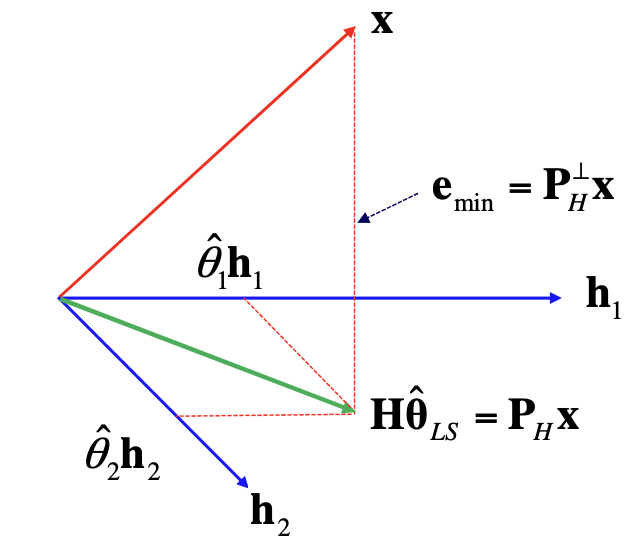
\includegraphics[width=0.5\linewidth]{Image/pdf 5/5.Geom_rapp_2.png}
    \label{fig:placeholder}
\end{figure}
\item Geometrical viewpoint of linear Least squares in \(R^3\):
\begin{align*}
\hat{\mathbf{s}}_{LS}
&= \mathbf{H}\hat{\boldsymbol{\theta}}_{LS}
 = \mathbf{P}_{\!H}\mathbf{x} \\[4pt]
\mathbf{e}_{\min}
&= \mathbf{x} - \hat{\mathbf{s}}_{LS}
 = \mathbf{x} - \mathbf{H}\hat{\boldsymbol{\theta}}_{LS}
 = \mathbf{P}_{\!H}^{\perp}\mathbf{x}
\end{align*}
\vspace{-1.5em}
\[
\mathbf{e}_{\min} \perp \mathbf{h}_{k} \quad \forall k
\quad\text{i.e.}\quad
\mathbf{e}_{\min} \perp \mathcal{R}(\mathbf{H})
\]

where \(\mathcal{R}(\mathbf{H})\) is the 2D subspace spanned by \(\mathbf{h}_{1}\) and \(\mathbf{h}_{2}\).

\item \textbf{Example}. we want to estimate the amplitude of a signal of known shape. In this case, the relationship between the signal of interest (SOI) and the unknown parameter is \textbf{linear}:
\begin{align*}
\mathbf{x}
&= \mathbf{s}(\boldsymbol{\theta}) + \mathbf{w}
 = A\mathbf{p} + \mathbf{w} \\[4pt]
\mathbf{s}(\boldsymbol{\theta})
&= \mathbf{H}\boldsymbol{\theta}
 = A\mathbf{p},
 \quad \text{where } \boldsymbol{\theta} = A
 \text{ and } \mathbf{H} = \mathbf{p} \text{ is perfectly known}
\end{align*}
\vspace{-1.25em}
\[
\hat{A}_{LS}
= \arg\min_{A} \left\| \mathbf{x} - A\mathbf{p} \right\|^{2}
\]

\item The \textbf{LS} method\(\rightarrow\) \underline{is a purely deterministic approach}.
\begin{align*}
\hat{A}_{LS}
&= \arg\min_{A} \left\| \mathbf{x} - A\mathbf{p} \right\|^{2} \\[4pt]
&= \mathbf{p}^{\#}\mathbf{x}
 = (\mathbf{p}^{H}\mathbf{p})^{-1}\mathbf{p}^{H}\mathbf{x} \\[4pt]
&= \frac{\mathbf{p}^{H}\mathbf{x}}{\mathbf{p}^{H}\mathbf{p}}
 = \frac{\mathbf{p}^{H}\mathbf{x}}{\lVert \mathbf{p} \rVert^{2}}
 = \frac{1}{E_{p}}\,\mathbf{p}^{H}\mathbf{x},
 \qquad \text{where } E_{p} \triangleq \lVert \mathbf{p} \rVert^{2}
 \text{ is the energy of vector } \mathbf{p}
\end{align*}
\vspace{-1.25em}
\begin{align*}
\hat{A}_{LS}
&= \frac{1}{E_{p}}\mathbf{p}^{H}\mathbf{x}
 = \frac{1}{E_{p}}\sum_{n=0}^{N-1} p_{n}^{*} x_{n}
 \;\longrightarrow\;
\text{FIR matched filter (matched to } \mathbf{p}\text{)}
\end{align*}
\vspace{-1.25em}
\begin{align*}
p_{n} = 1 \ \forall n
&\;\Rightarrow\;
E_{p} = N
\;\Rightarrow\;
\hat{A}_{LS}
 = \frac{1}{N}\sum_{n=0}^{N-1} x_{n}
 \;\longrightarrow\;
\text{Sample mean}
\end{align*}
\textbf{Example}: we want to reveal the presence of a \textbf{linear trend} in the observed data:
\[
X[n] = A + Bn + W[n], \qquad 0 \le n \le N-1
\]

\[
\underset{N \times 1}{\mathbf{X}}
=
\begin{bmatrix}
X[0] \\
X[1] \\
\vdots \\
X[N-1]
\end{bmatrix}
=
\begin{bmatrix}
1 & 0 \\
1 & 1 \\
\vdots & \vdots \\
1 & N-1
\end{bmatrix}
\begin{bmatrix}
A \\ B
\end{bmatrix}
+ \mathbf{W}
= \mathbf{H}\boldsymbol{\theta} + \mathbf{W}
\]

\[
\text{where}\quad
\underset{N \times 2}{\mathbf{H}} \triangleq
\begin{bmatrix}
1 & 0 \\
1 & 1 \\
\vdots & \vdots \\
1 & N-1
\end{bmatrix},
\qquad
\underset{2 \times 1}{\boldsymbol{\theta}} \triangleq
\begin{bmatrix}
A \\ B
\end{bmatrix}
\]

\[
\hat{\boldsymbol{\theta}}_{LS}
=
(\mathbf{H}^{H}\mathbf{H})^{-1}\mathbf{H}^{H}\mathbf{X}
=
\mathbf{H}^{\#}\mathbf{X}
\]

\begin{figure}[H]
    \centering
    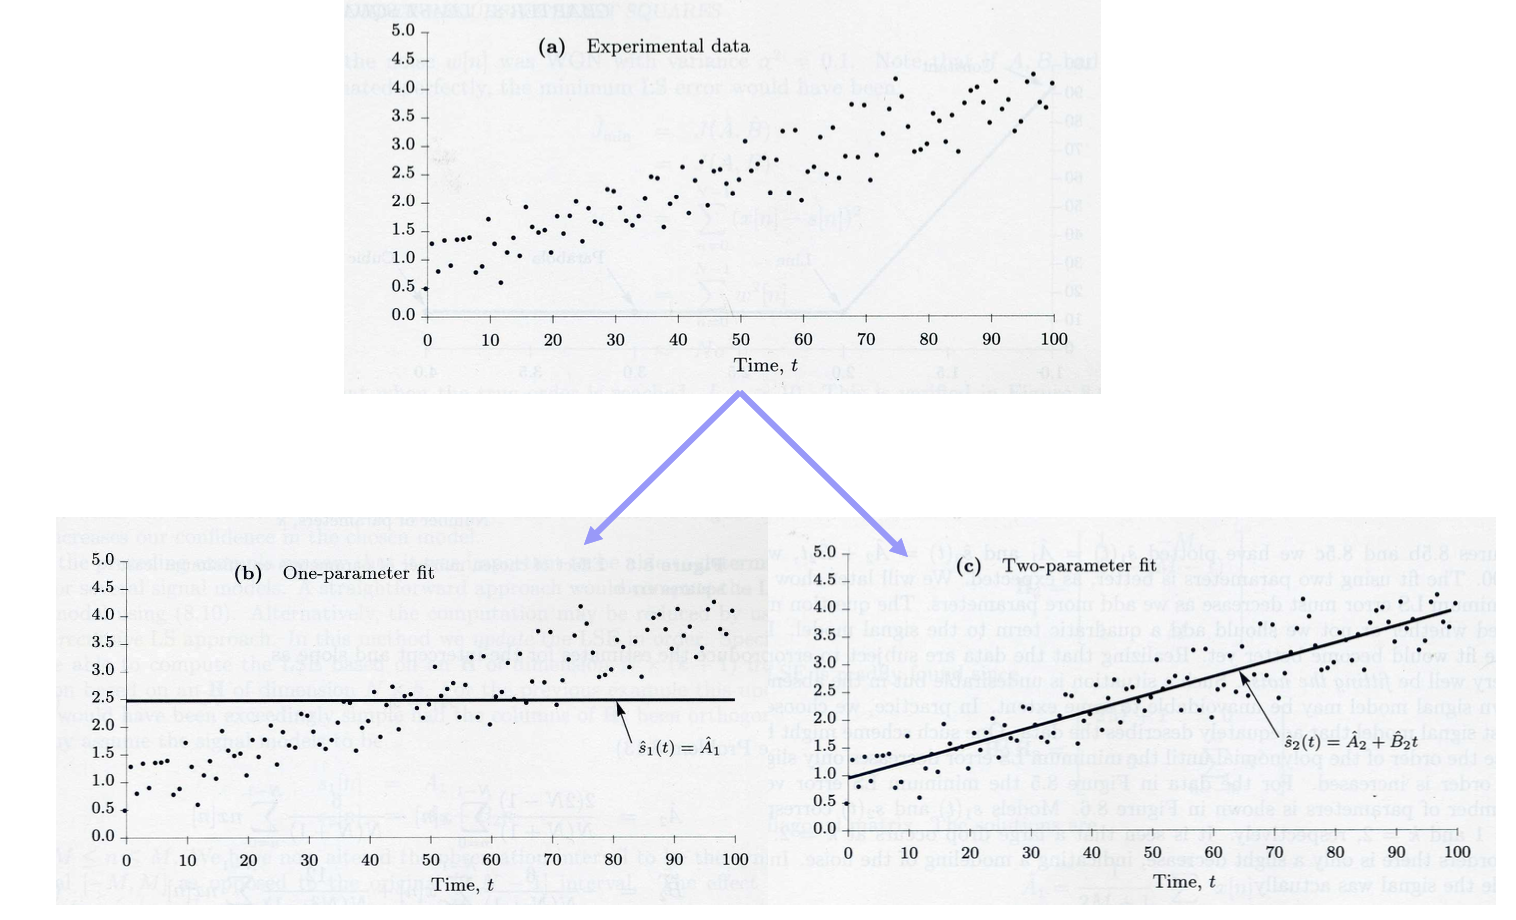
\includegraphics[width=0.75\linewidth]{Image/pdf 5/6.example_lin_mod.png}
    \label{fig:placeholder}
\end{figure}
\begin{align*}
\mathbf{H}^{\#}
&=
\left(
\begin{bmatrix}
1 & 0 \\
1 & 1 \\
\vdots & \vdots \\
1 & N-1
\end{bmatrix}^{\!H}
\begin{bmatrix}
1 & 0 \\
1 & 1 \\
\vdots & \vdots \\
1 & N-1
\end{bmatrix}
\right)^{-1}
\begin{bmatrix}
1 & 0 \\
1 & 1 \\
\vdots & \vdots \\
1 & N-1
\end{bmatrix}^{\!H} \\[6pt]
&=
\begin{bmatrix}
N & \displaystyle\sum_{k=0}^{N-1} k \\[6pt]
\displaystyle\sum_{k=0}^{N-1} k &
\displaystyle\sum_{k=0}^{N-1} k^{2}
\end{bmatrix}^{\!-1}
\begin{bmatrix}
1 & 1 & \cdots & 1 \\
0 & 1 & \cdots & N-1
\end{bmatrix} \\[8pt]
&=
\begin{bmatrix}
N & \dfrac{N(N-1)}{2} \\[6pt]
\dfrac{N(N-1)}{2} &
\dfrac{N(N-1)(2N-1)}{6}
\end{bmatrix}^{\!-1}
\begin{bmatrix}
1 & 1 & \cdots & 1 \\
0 & 1 & \cdots & N-1
\end{bmatrix}
\end{align*}
\begin{align*}
\mathbf{H}^{\#}
&=
\frac{2}{N}
\begin{bmatrix}
2 & \dfrac{N-1}{(N-1)(2N-1)/3} \\[3pt]
N-1 & \dfrac{(N-1)(2N-1)}{3}
\end{bmatrix}^{\!-1}
\begin{bmatrix}
1 & 1 & \cdots & 1 \\
0 & 1 & \cdots & N-1
\end{bmatrix} \\[6pt]
&=
\frac{6}{N(N-1)\left[2(2N-1)-3(N-1)\right]}
\begin{bmatrix}
\dfrac{(N-1)(2N-1)}{3} & -(N-1) \\
-(N-1) & 2
\end{bmatrix}
\begin{bmatrix}
1 & 1 & \cdots & 1 \\
0 & 1 & \cdots & N-1
\end{bmatrix}
\end{align*}

\begin{align*}
\hat{\boldsymbol{\theta}}_{LS}
&= \mathbf{H}^{\#}\mathbf{X} =
\frac{6}{N(N-1)(N+1)}
\begin{bmatrix}
\dfrac{(N-1)(2N-1)}{3} & -(N-1) \\[3pt]
-(N-1) & 2
\end{bmatrix}
\begin{bmatrix}
\displaystyle \sum_{n=0}^{N-1} X[n] \\[6pt]
\displaystyle \sum_{n=0}^{N-1} n\,X[n]
\end{bmatrix}
\end{align*}
\vspace{-1.5em}
\begin{align*}
\hat{A}_{LS}
&= \frac{2(2N-1)}{N(N+1)}
   \sum_{n=0}^{N-1} X[n]
   - \frac{6}{N(N+1)}
   \sum_{n=0}^{N-1} n\,X[n] \\[6pt]
\hat{B}_{LS}
&= -\,\frac{6}{N(N+1)}
   \sum_{n=0}^{N-1} X[n]
   + \frac{12}{N(N^{2}-1)}
   \sum_{n=0}^{N-1} n\,X[n]
\end{align*}

\item If the noise is AWGN, the LS estimators are also ML estimators.
\item As we already proved, the ML estimator of the Deterministic linear model is AWGN is efficient, therefore:
\begin{align*}
MSE\!\left\{\hat{A}_{ML}\right\}
&= CRB(A)
 = \sigma_W^{2}
   \big[\left(\mathbf{H}^{H}\mathbf{H}\right)^{-1}\big]_{1,1}
 = \frac{2(2N-1)}{N(N+1)}\,\sigma_W^{2}
 \propto \frac{1}{N}
\\[8pt]
MSE\!\left\{\hat{B}_{ML}\right\}
&= CRB(B)
 = \sigma_W^{2}
   \big[\left(\mathbf{H}^{H}\mathbf{H}\right)^{-1}\big]_{2,2}
 = \frac{12}{N(N^{2}-1)}\,\sigma_W^{2}
 \propto \frac{1}{N^{3}}
\end{align*}
\item This result suggest that we can estimate more accurately the slope \(B\) than the parameter \(A\), since the observed data are more strongly affected by \(B\).
\begin{figure}[H]
    \centering
    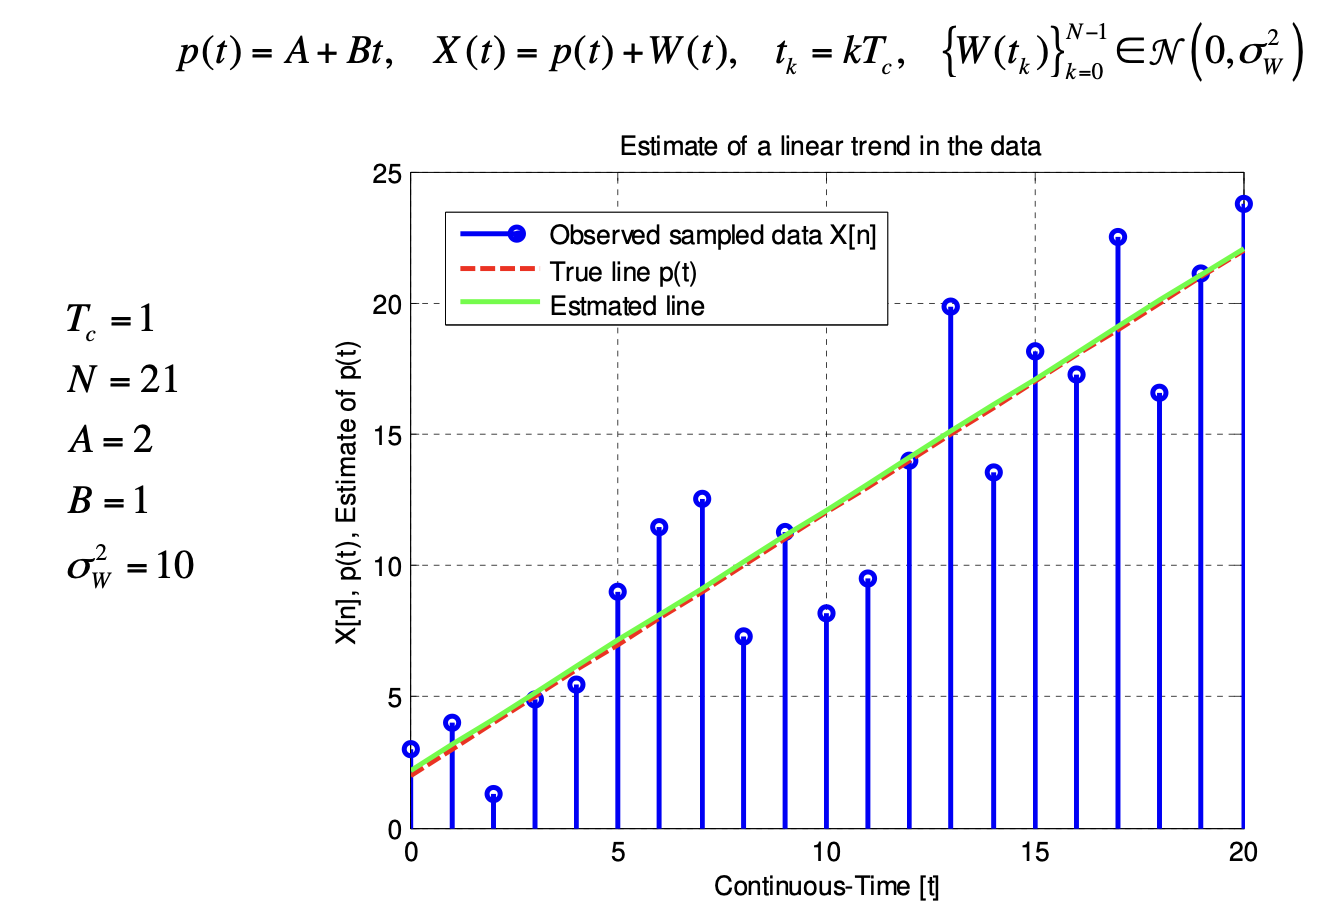
\includegraphics[width=0.65\linewidth]{Image/pdf 5/7.LM_graph.png}
    \label{fig:placeholder}
\end{figure}
\begin{figure}[H]
    \centering
    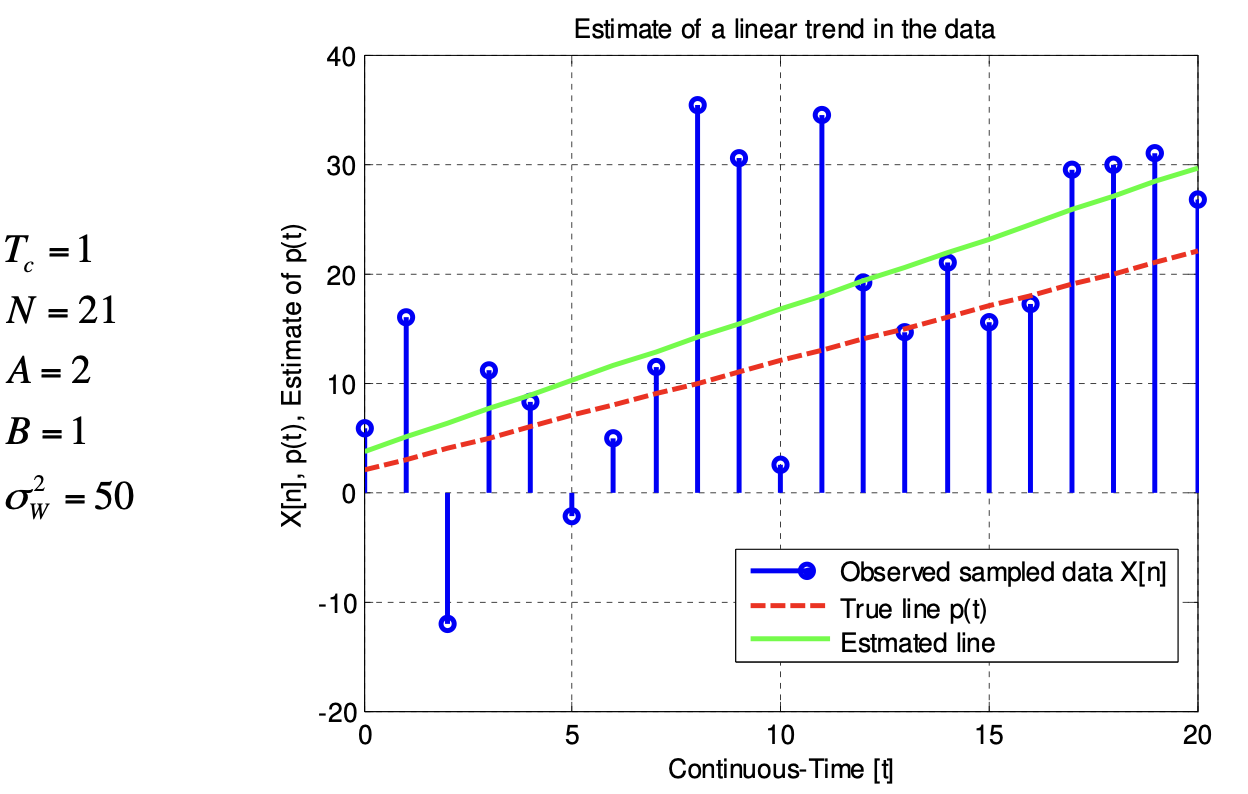
\includegraphics[width=0.65\linewidth]{Image/pdf 5/8.LM_graph_1.png}
    \label{fig:placeholder}
\end{figure}
\begin{figure}[H]
    \centering
    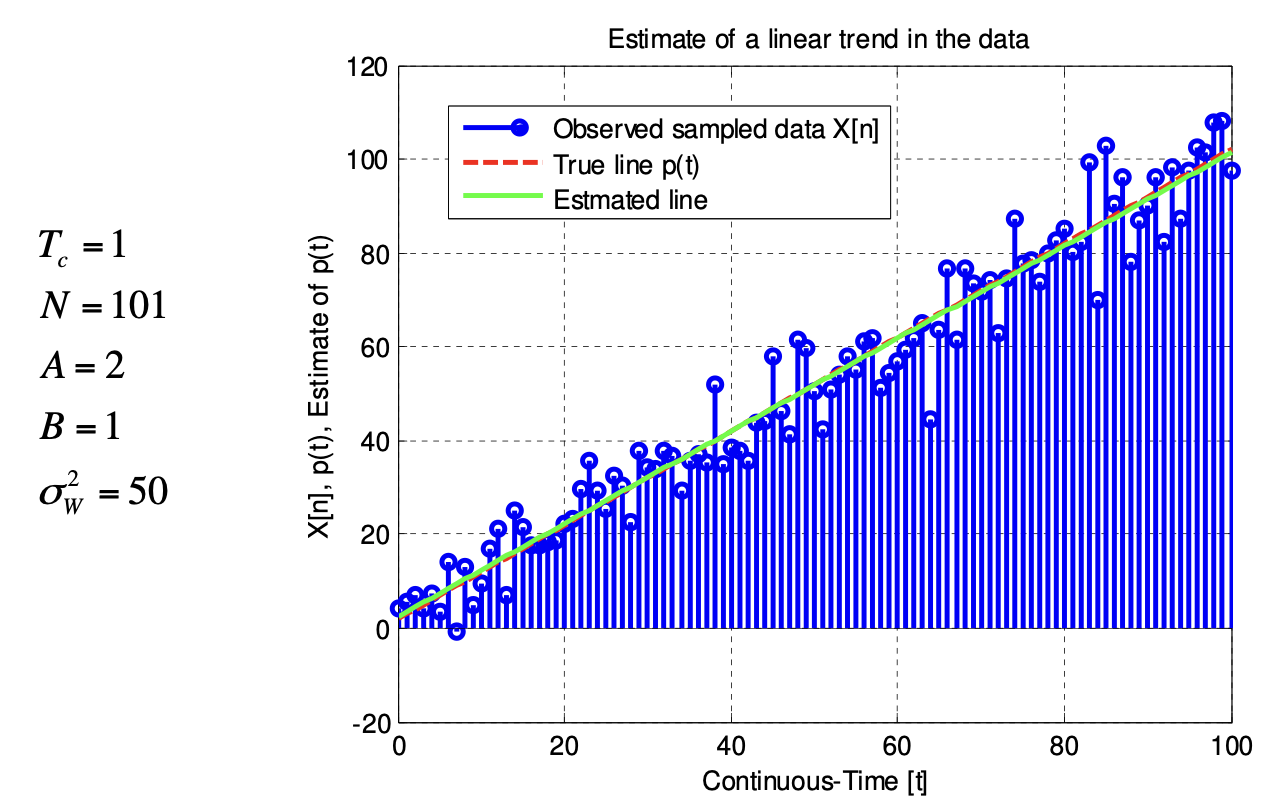
\includegraphics[width=0.65\linewidth]{Image/pdf 5/9.LM_graph_2.png}
    \label{fig:placeholder}
\end{figure}

\item \textbf{Example}: we want to estimate the amplitude and phase of a sinusoid in AWGN:
\newpage
\begin{align*}
X[n] &= \frac{A}{\sqrt{2B}}\cos(2\pi F_{0} n + \theta) + W[n]\\
 &= \frac{A}{\sqrt{2B}}\cos(\theta)\cos(2\pi F_{0} n)
 - \frac{A}{\sqrt{2B}}\sin(\theta)\sin(2\pi F_{0} n)
 + W[n], \qquad 0 \le n \le N-1
\end{align*}
\[
\begin{cases}
\theta_{1} \triangleq \frac{A}{\sqrt{2B}}\cos(\theta),\qquad\mathbf{h}_{1} \triangleq
\big[\,1,\ \cos(2\pi F_{0}),\ \ldots,\ \cos(2\pi F_{0}(N-1))\,\big]^{T}\\
\theta_{2} \triangleq -\frac{A}{\sqrt{2B}}\sin(\theta) \qquad \mathbf{h}_{2} \triangleq
\big[\,0,\ \sin(2\pi F_{0}),\ \ldots,\ \sin(2\pi F_{0}(N-1))\,\big]^{T}
\end{cases}\]
\[
\mathbf{X} = \theta_{1}\mathbf{h}_{1} + \theta_{2}\mathbf{h}_{2} + \mathbf{W}
= \mathbf{H}\boldsymbol{\theta} + \mathbf{W},
\qquad
F_{0} \triangleq \frac{f_{0}}{2B} \ \text{(digital frequency)}
\]

\item This is the so-called "\textbf{Deterministic Linear Model}":
\[
\mathbf{X} = \mathbf{H}\boldsymbol{\theta} + \mathbf{W},
\qquad
\text{where}\quad
\underset{2 \times 1}{\boldsymbol{\theta}}
\triangleq
\begin{bmatrix}
\theta_{1} \\
\theta_{2}
\end{bmatrix},
\quad
\underset{N \times 2}{\mathbf{H}}
\triangleq
\big[\, \mathbf{h}_{1}\ \ \mathbf{h}_{2} \,\big]
\]
\item Where: 
\[
\boldsymbol{\theta}
\triangleq
\begin{bmatrix}
\theta_{1} \\
\theta_{2}
\end{bmatrix}
=
\mathbf{g}(\mathbf{q})
=
\begin{bmatrix}
\dfrac{A}{\sqrt{2B}}\cos(\theta)\\[5pt]
-\dfrac{A}{\sqrt{2B}}\sin(\theta)
\end{bmatrix},
\qquad
\mathbf{q}
\triangleq
\begin{bmatrix}
A \\
\theta
\end{bmatrix}
\]
\item \textbf{Problem}: estimate \(\theta\), given the observed data vector \(\textbf{X}\), assuming that \textbf{H} is \textbf{a-priori} known.
\item Once we have derived the ML estimate of vector \(\theta\), the ML estimate of the vector \(\textbf{q}\) can be immediately derived thanks to the \textbf{invariance property} of the ML estimate:
\[
\boldsymbol{\theta} = \mathbf{g}(\mathbf{q}) \text{ invertible: }
\quad
\mathbf{q} = \mathbf{g}^{-1}(\boldsymbol{\theta})
\;\Rightarrow\;
\hat{\mathbf{q}}_{ML}
= \mathbf{g}^{-1}(\hat{\boldsymbol{\theta}}_{ML})
\]

\[
\mathbf{q} =
\begin{bmatrix}
A \\[2pt]
\theta
\end{bmatrix}
= \mathbf{g}^{-1}(\boldsymbol{\theta})
=
\begin{bmatrix}
\sqrt{2B}\,\sqrt{\theta_{1}^{2} + \theta_{2}^{2}} \\[4pt]
-\arctan\!\left(\dfrac{\theta_{2}}{\theta_{1}}\right)
\end{bmatrix}
\;\Rightarrow\;
\begin{cases}
\hat{A}_{ML}
= \sqrt{2B}\,\sqrt{\hat{\theta}_{1,ML}^{2} + \hat{\theta}_{2,ML}^{2}} \\[6pt]
\hat{\theta}_{ML}
= -\arctan\!\left(\dfrac{\hat{\theta}_{2,ML}}{\hat{\theta}_{1,ML}}\right)
\end{cases}
\]
\item It is worth observing that in the case we want to estimate the parameters of a sinusoid of unknown aplitude, phase and \textbf{frequency}, matrix \textbf{H} is not perfectly known, but it is a known function of the unknown parameter \(F_0\), i.e. it is parametrized by the unknown parameter \(F_0\):
\[
\underset{N \times 1}{\mathbf{X}}
= \mathbf{H}(F_{0})\boldsymbol{\theta} + \mathbf{W}
= \sum_{i=1}^{p} \theta_{i}\mathbf{h}_{i}(F_{0}) + \mathbf{W}
\]

\[
\underset{N \times 2}{\mathbf{H}}(F_{0})
= \big[\,\mathbf{h}_{1}(F_{0}) \;\; \mathbf{h}_{2}(F_{0})\,\big]
=
\begin{bmatrix}
1 & 0 \\
\cos(2\pi F_{0}) & \sin(2\pi F_{0}) \\
\vdots & \vdots \\
\cos\big(2\pi F_{0}(N-1)\big) &
\sin\big(2\pi F_{0}(N-1)\big)
\end{bmatrix}
\]

\item Assume first sta \(F_0\) is \underline{known} and we want to estimate \textbf{amplitude} and \textbf{phase}:

\[
\hat{\boldsymbol{\theta}}_{ML}
=
\begin{bmatrix}
\hat{\theta}_{1,ML} \\
\hat{\theta}_{2,ML}
\end{bmatrix}
=
\mathbf{H}^{\#}\mathbf{x}
=
(\mathbf{H}^{T}\mathbf{H})^{-1}\mathbf{H}^{T}\mathbf{x}
\;\Rightarrow\;
\begin{cases}
\hat{A}_{ML}
= \sqrt{2B}\,\sqrt{\hat{\theta}_{1,ML}^{2} + \hat{\theta}_{2,ML}^{2}} \\[6pt]
\hat{\theta}_{ML}
= -\arctan\!\left(\dfrac{\hat{\theta}_{2,ML}}{\hat{\theta}_{1,ML}}\right)
\end{cases}
\]

\[
\mathbf{H} = [\,\mathbf{h}_{1}\ \mathbf{h}_{2}\,], \quad
\text{where}\quad
\begin{cases}
\mathbf{h}_{1} \triangleq
\big[\,1,\ \cos(2\pi F_{0}),\ \ldots,\ \cos(2\pi F_{0}(N-1))\,\big]^{T}\\
\mathbf{h}_{2} \triangleq
\big[\,0,\ \sin(2\pi F_{0}),\ \ldots,\ \sin(2\pi F_{0}(N-1))\,\big]^{T}
\end{cases}
\]
\begin{align*}
\mathbf{H}^{\#}
&= (\mathbf{H}^{T}\mathbf{H})^{-1}\mathbf{H}^{T}
 = \begin{bmatrix}
\mathbf{h}_{1}^{T} \\
\mathbf{h}_{2}^{T}
\end{bmatrix}
[\,\mathbf{h}_{1}\ \mathbf{h}_{2}\,]^{-1}
\begin{bmatrix}
\mathbf{h}_{1}^{T} \\
\mathbf{h}_{2}^{T}
\end{bmatrix}  \\[4pt]
&= \begin{bmatrix}
\mathbf{h}_{1}^{T}\mathbf{h}_{1} & \mathbf{h}_{1}^{T}\mathbf{h}_{2} \\
\mathbf{h}_{2}^{T}\mathbf{h}_{1} & \mathbf{h}_{2}^{T}\mathbf{h}_{2}
\end{bmatrix}^{-1}
\begin{bmatrix}
\mathbf{h}_{1}^{T} \\
\mathbf{h}_{2}^{T}
\end{bmatrix}
= \begin{bmatrix}
N/2 & 0 \\
0 & N/2
\end{bmatrix}^{-1}
\begin{bmatrix}
\mathbf{h}_{1}^{T} \\
\mathbf{h}_{2}^{T}
\end{bmatrix}
= \frac{2}{N}
\begin{bmatrix}
\mathbf{h}_{1}^{T} \\
\mathbf{h}_{2}^{T}
\end{bmatrix}
\end{align*}
\item In fact, if \(N\gg1\) we have:
\begin{align*}
\mathbf{h}_{1}^{T}\mathbf{h}_{1}
&= \lVert \mathbf{h}_{1} \rVert^{2}
 = \sum_{n=0}^{N-1} \cos^{2}(2\pi F_{0} n)
 = \sum_{n=0}^{N-1} \left(\frac{1}{2} + \frac{1}{2}\cos(4\pi F_{0} n)\right) \\[4pt]
&= \frac{N}{2}
   \left(1 + \frac{1}{N}\sum_{n=0}^{N-1}\cos(4\pi F_{0} n)\right)
 \approx \frac{N}{2}
\end{align*}
\vspace{-1.5em}
\begin{align*}
\mathbf{h}_{2}^{T}\mathbf{h}_{2}
&= \lVert \mathbf{h}_{2} \rVert^{2}
 = \sum_{n=0}^{N-1} \sin^{2}(2\pi F_{0} n)
 = \sum_{n=0}^{N-1} \left(\frac{1}{2} - \frac{1}{2}\cos(4\pi F_{0} n)\right) \\[4pt]
&= \frac{N}{2}
   \left(1 - \frac{1}{N}\sum_{n=0}^{N-1}\cos(4\pi F_{0} n)\right)
 \approx \frac{N}{2}
\end{align*}
\vspace{-1.5em}
\begin{align*}
\mathbf{h}_{1}^{T}\mathbf{h}_{2}
&= \mathbf{h}_{2}^{T}\mathbf{h}_{1}
 = \sum_{n=0}^{N-1} \cos(2\pi F_{0} n)\sin(2\pi F_{0} n)
 = \frac{1}{2}\sum_{n=0}^{N-1}\cos(4\pi F_{0} n)
 \approx 0
\end{align*}

\item The ML/Linear LS estimate of vector \(\theta\) and its MSE are finally derived as:
\begin{align*}
\hat{\boldsymbol{\theta}}_{ML}
&=
\begin{bmatrix}
\hat{\theta}_{1,ML} \\
\hat{\theta}_{2,ML}
\end{bmatrix}
= \mathbf{H}^{\#}\mathbf{x}
= \frac{2}{N}
\begin{bmatrix}
\mathbf{h}_{1}^{T} \\
\mathbf{h}_{2}^{T}
\end{bmatrix}\mathbf{x}
=
\begin{bmatrix}
\displaystyle \frac{2}{N}\sum_{n=0}^{N-1} X[n]\cos(2\pi F_{0} n) \\[8pt]
\displaystyle \frac{2}{N}\sum_{n=0}^{N-1} X[n]\sin(2\pi F_{0} n)
\end{bmatrix}
\end{align*}
\vspace{-1.5em}
\begin{align*}
MSE\!\left\{\hat{\boldsymbol{\theta}}_{ML}\right\}
&= \sigma_W^{2}(\mathbf{H}^{T}\mathbf{H})^{-1}
 = \sigma_W^{2}
   \begin{bmatrix}
   N/2 & 0 \\
   0 & N/2
   \end{bmatrix}^{-1}
 = \begin{bmatrix}
   \dfrac{2\sigma_W^{2}}{N} & 0 \\
   0 & \dfrac{2\sigma_W^{2}}{N}
   \end{bmatrix}
 = \frac{2\sigma_W^{2}}{N}\,\mathbf{I}
\end{align*}

\[
\begin{cases}
\hat{A}_{ML}
= \sqrt{2B}\,\sqrt{\hat{\theta}_{1,ML}^{2} + \hat{\theta}_{2,ML}^{2}} \\[6pt]
\hat{\theta}_{ML}
= -\arctan\!\left(\dfrac{\hat{\theta}_{2,ML}}{\hat{\theta}_{1,ML}}\right)
\end{cases}
\]
The estimator is therefore consistent since \(MSE \to 0\) as \(N \to \infty\).
\[
\hat{\boldsymbol{\theta}}_{ML}
= \hat{\boldsymbol{\theta}}_{LS}
= \mathbf{H}^{\#}\mathbf{x}
=
\begin{bmatrix}
\dfrac{2}{N}\displaystyle\sum_{n=0}^{N-1} X[n]\cos(2\pi F_{0} n) \\[8pt]
\dfrac{2}{N}\displaystyle\sum_{n=0}^{N-1} X[n]\sin(2\pi F_{0} n)
\end{bmatrix}
\]

\[
\begin{cases}
\displaystyle
\hat{A}_{ML}
= \dfrac{2\sqrt{2B}}{N}
\sqrt{
\left(\displaystyle\sum_{n=0}^{N-1} X[n]\cos(2\pi F_{0} n)\right)^{2}
+
\left(\displaystyle\sum_{n=0}^{N-1} X[n]\sin(2\pi F_{0} n)\right)^{2}
} \\[14pt]
\displaystyle
\hat{\theta}_{ML}
= -\arctan\!\left(
\dfrac{\displaystyle\sum_{n=0}^{N-1} X[n]\sin(2\pi F_{0} n)}
      {\displaystyle\sum_{n=0}^{N-1} X[n]\cos(2\pi F_{0} n)}
\right)
\end{cases}
\]
Coincidono con quelle già derivate.
\end{itemize}
\subsubsection{Non-Linear Least Squares (NLLS)}

\begin{itemize}
    \item If the frequency \(F_0\) is \underline{unknown}, \textbf{H} is also unknown. To be more precise, \textbf{H} is a known function of the unknown \(F_0\):
\[
\big(\hat{\boldsymbol{\theta}}_{ML},\hat{F}_{0,ML}\big)
= \arg\min_{\boldsymbol{\theta},F_{0}} J(\boldsymbol{\theta},F_{0})
= \arg\min_{\boldsymbol{\theta},F_{0}}
\big\|\mathbf{x} - \mathbf{H}(F_{0})\boldsymbol{\theta}\big\|^{2}
\]

\[
\hat{\boldsymbol{\theta}}_{ML}(F_{0})
= \hat{\boldsymbol{\theta}}_{LS}(F_{0})
= (\mathbf{H}^{T}\mathbf{H})^{-1}\mathbf{H}^{T}\mathbf{x}
= \mathbf{H}^{\#}\mathbf{x}
\]

\[
\underset{N\times 2}{\mathbf{H}(F_{0})}
= [\,\mathbf{h}_{1}(F_{0})\ \mathbf{h}_{2}(F_{0})\,]
=
\begin{bmatrix}
1 & 0 \\
\cos(2\pi F_{0}) & \sin(2\pi F_{0}) \\
\vdots & \vdots \\
\cos\big(2\pi F_{0}(N-1)\big) &
\sin\big(2\pi F_{0}(N-1)\big)
\end{bmatrix}^{T}
\]

    \item \textbf{ML estimate} of \(F_0\) coincides with the \textbf{Non-Linear Least Squares} estimate: it is the value that minimizes the energy of the error between the data \textbf{x} and the model. It is nonlinear since the signal depends on \(F_0\) in a nonlinear fashion.
    \item Once we have derived the ML (i.e. the linear LS) estimate of \(\theta\), we insert the estimate in the functional \(J(.)\) to be minimized and derive the estimate of \(F_0\) by minimizing the "compressed" functional w.r.t. \(F_0\):
\begin{align*}
\hat{F}_{0,ML}
= \hat{F}_{0,NLLS}
&= \arg\min_{F_{0}} J\big(\hat{\boldsymbol{\theta}}_{ML}(F_{0}),F_{0}\big)
 = \arg\min_{F_{0}}\big\|\mathbf{x}-\mathbf{H}(F_{0})\hat{\boldsymbol{\theta}}_{ML}(F_{0})\big\|^{2} \\[4pt]
&= \arg\min_{F_{0}}\big\|\mathbf{x}-\mathbf{H}(F_{0})\mathbf{H}^{\#}(F_{0})\mathbf{x}\big\|^{2} \\[4pt]
&= \arg\min_{F_{0}}\big\|(\mathbf{I}-\mathbf{H}(F_{0})\mathbf{H}^{\#}(F_{0}))\mathbf{x}\big\|^{2} = \arg\min_{F_{0}}\big\|(\mathbf{I}-\mathbf{P}_{H}(F_{0}))\mathbf{x}\big\|^{2} \\[4pt]
&= \arg\min_{F_{0}}\big\|\mathbf{P}_{H}^{\perp}(F_{0})\mathbf{x}\big\|^{2} = \arg\max_{F_{0}}\big\|\mathbf{P}_{H}(F_{0})\mathbf{x}\big\|^{2}
\end{align*}
\[
\hat{F}_{0,ML}
= \hat{F}_{0,NLLS}
= \arg\max_{F_{0}}
\big\|\mathbf{P}_{H}(F_{0})\mathbf{x}\big\|^{2}
\]

\item The ML/NLLS estimate of \(F_0\) is the value that maximizes the energy of the component of the data vector \textbf{x} onto the subspace generated by the columns of matrix \textbf{H}.
\item It can shown that this is equivalent to find the location of the maximum in the \textbf{Periodigram} of vector \textbf{x}.
\item The projection matrix of \textbf{H} is given by:
\[
\mathbf{P}_{H}
= \mathbf{H}\mathbf{H}^{\#}
= [\,\mathbf{h}_{1}\ \mathbf{h}_{2}\,]\,
\frac{2}{N}
\begin{bmatrix}
\mathbf{h}_{1}^{T} \\
\mathbf{h}_{2}^{T}
\end{bmatrix}
= \frac{2}{N}
[\,\mathbf{h}_{1}\ \mathbf{h}_{2}\,]
\begin{bmatrix}
\mathbf{h}_{1}^{T} \\
\mathbf{h}_{2}^{T}
\end{bmatrix}
= \mathbf{P}_{H}^{T}
\]
\[
\mathbf{P}_{H}(F_{0}) = \frac{2}{N}
[\,\mathbf{h}_{1}\ \mathbf{h}_{2}\,]
\begin{bmatrix}
\mathbf{h}_{1}^{T} \\
\mathbf{h}_{2}^{T}
\end{bmatrix}
\]
\vspace{-1.5em}
\begin{align*}
\big\|\mathbf{P}_{H}(F_{0})\mathbf{x}\big\|^{2}
&= (\mathbf{P}_{H}\mathbf{x})^{T}(\mathbf{P}_{H}\mathbf{x})
 = \mathbf{x}^{T}\mathbf{P}_{H}^{T}\mathbf{P}_{H}\mathbf{x}
 = \mathbf{x}^{T}\mathbf{P}_{H}\mathbf{x} \\[4pt]
&= \frac{2}{N}\mathbf{x}^{T}
[\,\mathbf{h}_{1}\ \mathbf{h}_{2}\,]
\begin{bmatrix}
\mathbf{h}_{1}^{T} \\
\mathbf{h}_{2}^{T}
\end{bmatrix}
\mathbf{x}
= \frac{2}{N}
\begin{bmatrix}
\mathbf{h}_{1}^{T}\mathbf{x} \\
\mathbf{h}_{2}^{T}\mathbf{x}
\end{bmatrix}^{T}
\begin{bmatrix}
\mathbf{h}_{1}^{T}\mathbf{x} \\
\mathbf{h}_{2}^{T}\mathbf{x}
\end{bmatrix} \\[4pt]
&= \frac{2}{N}
\left(\big(\mathbf{h}_{1}^{T}\mathbf{x}\big)^{2}
      + \big(\mathbf{h}_{2}^{T}\mathbf{x}\big)^{2}\right) \\[4pt]
&= \frac{2}{N}
\left|(\mathbf{h}_{1}-j\mathbf{h}_{2})^{T}\mathbf{x}\right|^{2}
= \frac{2}{N}
\left|\sum_{n=0}^{N-1}
X_{n}\big(\cos(2\pi F_{0}n)-j\sin(2\pi F_{0}n)\big)\right|^{2} \\[4pt]
&= 2\cdot \frac{1}{N}
\left|\sum_{n=0}^{N-1} X_{n}e^{-j2\pi F_{0}n}\right|^{2}
\;\longrightarrow\; \text{Periodogram of } \mathbf{x}
\end{align*}

\item Once we have derived the NLLS estimate of \(F_0\) (which in AWGN coincides with the ML estimator), we can calculate \textbf{H} and derive the ML/LS estimate of \(\theta\):
\[
\underset{N\times 2}{\mathbf{H}}(\hat{F}_{0,ML})
= \big[\,\mathbf{h}_{1}(\hat{F}_{0,ML})\ \mathbf{h}_{2}(\hat{F}_{0,ML})\,\big]
=
\begin{bmatrix}
1 & 0 \\
\cos\!\big(2\pi \hat{F}_{0,ML}\big) & \sin\!\big(2\pi \hat{F}_{0,ML}\big) \\
\vdots & \vdots \\
\cos\!\big(2\pi \hat{F}_{0,ML}(N-1)\big) &
\sin\!\big(2\pi \hat{F}_{0,ML}(N-1)\big)
\end{bmatrix}
\]

\[
\mathbf{H}^{\#}(\hat{F}_{0,ML})
= \big(\mathbf{H}^{T}(\hat{F}_{0,ML})\,\mathbf{H}(\hat{F}_{0,ML})\big)^{-1}
   \mathbf{H}^{T}(\hat{F}_{0,ML})
\]

\item And finally, the ML estimates of \(A\) and \(\theta\):
\[
\hat{\boldsymbol{\theta}}_{ML}
= \hat{\boldsymbol{\theta}}_{LS}
= \mathbf{H}^{\#}\big(\hat{F}_{0,ML}\big)\mathbf{x}
\quad\Longrightarrow\quad
\begin{cases}
\displaystyle
\hat{A}_{ML}
= \sqrt{2B}\,\sqrt{\hat{\theta}_{1,ML}^{2} + \hat{\theta}_{2,ML}^{2}} \\[8pt]
\displaystyle
\hat{\theta}_{ML}
= -\arctan\!\left(\dfrac{\hat{\theta}_{2,ML}}{\hat{\theta}_{1,ML}}\right)
\end{cases}
\]

\item It is \textbf{important} to stress that the location of the maximum of th \textbf{periodogram} is no more ML estimate of \(F_0\) if the noise is not Gaussian and/or not white, but it is still the NLLS estimate of \(F_0\), whatever is the noise distribution and/or the noise color(i.e the noise PSD).
\item For the same reason, the output of the \textbf{Matched Filter}(matched to the know signal shape \textbf{s}) is no more the ML estimate of the amplitude \(A\) if the noise is not Gaussian and/or not white, but it is still the linear LS estimate of \(A\), whatever is the noise distribution and/or the noise color.
\end{itemize}
\subsection{The Deterministic Linear Model in Colored Gaussian Noise}
\begin{itemize}
    \item \textbf{Assumption}: the noise is \underline{real}, Gaussian, but \textbf{correlated} with known covariance matrix \textbf{R}:
\[
f_{\mathbf{X}}(\mathbf{x};\boldsymbol{\theta})
= \frac{1}{\sqrt{(2\pi)^{N}\,|\mathbf{R}|}}
   \exp\!\left(
   -\frac{1}{2}
   (\mathbf{x}-\mathbf{H}\boldsymbol{\theta})^{T}
   \mathbf{R}^{-1}
   (\mathbf{x}-\mathbf{H}\boldsymbol{\theta})
   \right)
\]

    \item The \textbf{log-likelihood Function} is given by:
\[
\ln L(\boldsymbol{\theta})
= \ln f_{\mathbf{X}}(\mathbf{x};\boldsymbol{\theta})
= \kappa
 - \frac{1}{2}
   (\mathbf{x}-\mathbf{H}\boldsymbol{\theta})^{T}
   \mathbf{R}^{-1}
   (\mathbf{x}-\mathbf{H}\boldsymbol{\theta})
\]

    \item The \textbf{ML estimate} is obtained by solving the following problem:
\begin{align*}
\hat{\boldsymbol{\theta}}_{ML}
&= \arg\max_{\boldsymbol{\theta}} \ln L(\boldsymbol{\theta})
= \arg\min_{\boldsymbol{\theta}}
(\mathbf{x}-\mathbf{H}\boldsymbol{\theta})^{T}
\mathbf{R}^{-1}
(\mathbf{x}-\mathbf{H}\boldsymbol{\theta})\\[4pt]
&= \arg\min_{\boldsymbol{\theta}}
\big\|\mathbf{x}-\mathbf{H}\boldsymbol{\theta}\big\|^{2}_{\mathbf{R}^{-1}}
= \hat{\boldsymbol{\theta}}_{WLS}
\qquad \text{(Weighted Least Squares)}
\end{align*}

    \item In general, the \textbf{WLS estimate} is given by:
    
    
    \item The weighting matrix \textbf{W} has the purpose to introduce different weights for different data, e.g. because some of them could be more noisy or less reliable.
    \item  \textit{Example}:

        \[
\mathbf{R} =
\begin{bmatrix}
\sigma_0^{2} & 0 & \cdots & 0 \\
0 & \sigma_1^{2} & \cdots & 0 \\
\vdots & \vdots & \ddots & \vdots \\
0 & 0 & \cdots & \sigma_{N-1}^{2}
\end{bmatrix}
\;\Rightarrow\;
\mathbf{W} = \mathbf{R}^{-1} =
\begin{bmatrix}
1/\sigma_0^{2} & 0 & \cdots & 0 \\
0 & 1/\sigma_1^{2} & \cdots & 0 \\
\vdots & \vdots & \ddots & \vdots \\
0 & 0 & \cdots & 1/\sigma_{N-1}^{2}
\end{bmatrix}
\]
\[
\hat{\boldsymbol{\theta}}_{WLS}
= \arg\min_{\boldsymbol{\theta}}
(\mathbf{x}-\mathbf{H}\boldsymbol{\theta})^{T}
\mathbf{W}
(\mathbf{x}-\mathbf{H}\boldsymbol{\theta})
= \arg\min_{\boldsymbol{\theta}}
\sum_{k=0}^{N-1}
\frac{1}{\sigma_k^{2}}
\left(
x_k - \sum_{i=1}^{p}\theta_i h_{i,k}
\right)^{2}
\]
    \item The more noisy data are weighted less, since they are less reliable.
    \item The \textbf{ML} estimate of \(\theta\) in \underline{correlated} additive Gaussian noise is still, \textbf{linear},\textbf{unbiased},\textbf{Gaussian},\textbf{efficient} and \textbf{consistent}:
\begin{align*}
&\hat{\boldsymbol{\theta}}_{ML}
= \big(\mathbf{H}^{T}\mathbf{R}^{-1}\mathbf{H}\big)^{-1}
  \mathbf{H}^{T}\mathbf{R}^{-1}\mathbf{x}\\[3pt]
&E\{\hat{\boldsymbol{\theta}}_{ML}\}
= \big(\mathbf{H}^{T}\mathbf{R}^{-1}\mathbf{H}\big)^{-1}
  \mathbf{H}^{T}\mathbf{R}^{-1}E\{\mathbf{X}\}
= \big(\mathbf{H}^{T}\mathbf{R}^{-1}\mathbf{H}\big)^{-1}
  \mathbf{H}^{T}\mathbf{R}^{-1}\mathbf{H}\boldsymbol{\theta}
= \boldsymbol{\theta}\\[3pt]
&MSE\{\hat{\boldsymbol{\theta}}_{ML}\}
= CRB(\boldsymbol{\theta})
= \big(\mathbf{H}^{T}\mathbf{R}^{-1}\mathbf{H}\big)^{-1}\\[3pt]
&\hat{\boldsymbol{\theta}}_{ML}
\in \mathcal{N}\big(\boldsymbol{\theta},CRB(\boldsymbol{\theta})\big)
\end{align*}

\item \textbf{Proof}: We can easily derive the \textbf{ML estimator} of \(\theta\) in \textbf{correlated noise} by applying the previous results to the "whitened" data \textbf{Z}:
\[
\text{Whitening:}\quad
\mathbf{Z} \triangleq \mathbf{R}^{-1/2}\mathbf{X}
= \mathbf{R}^{-1/2}\mathbf{H}\boldsymbol{\theta}
  + \mathbf{R}^{-1/2}\mathbf{W}
= \tilde{\mathbf{H}}\boldsymbol{\theta}
  + \tilde{\mathbf{W}}
\;\Rightarrow\;
\mathbf{Z} \in \mathcal{N}\big(\tilde{\mathbf{H}}\boldsymbol{\theta},\mathbf{I}\big)
\]
\begin{align*}
E\{\tilde{\mathbf{W}}\tilde{\mathbf{W}}^{T}\}
&= E\{(\mathbf{R}^{-1/2}\mathbf{W})(\mathbf{R}^{-1/2}\mathbf{W})^{T}\}
= E\{\mathbf{R}^{-1/2}\mathbf{W}\mathbf{W}^{T}(\mathbf{R}^{-1/2})^{T}\}\\[3pt]
&= \mathbf{R}^{-1/2}E\{\mathbf{W}\mathbf{W}^{T}\}(\mathbf{R}^{-1/2})^{T}
= \mathbf{R}^{-1/2}\mathbf{R}\mathbf{R}^{-1/2}
= \mathbf{R}^{-1/2}\mathbf{R}^{1/2}\mathbf{R}^{1/2}\mathbf{R}^{-1/2}
= \mathbf{I}
\;\Rightarrow\;
\sigma_{\tilde{W}}^{2} = 1
\end{align*}
\[
\text{since } \mathbf{R} = \mathbf{R}^{T}
\;\Rightarrow\;
\mathbf{R}^{-1/2} = (\mathbf{R}^{-1/2})^{T}
\]
\item The \textbf{ML estimator} of \(\theta\) for \textbf{correlated noise} is immediately derived:
\begin{align*}
\hat{\boldsymbol{\theta}}_{ML}
&= \tilde{\mathbf{H}}^{\#}\mathbf{Z}
 = \big(\tilde{\mathbf{H}}^{T}\tilde{\mathbf{H}}\big)^{-1}
   \tilde{\mathbf{H}}^{T}\mathbf{Z}
 \quad\big|\;
   \tilde{\mathbf{H}} = \mathbf{R}^{-1/2}\mathbf{H},
   \ \mathbf{Z} = \mathbf{R}^{-1/2}\mathbf{X} \\[4pt]
&= \big((\mathbf{R}^{-1/2}\mathbf{H})^{T}\mathbf{R}^{-1/2}\mathbf{H}\big)^{-1}
   (\mathbf{R}^{-1/2}\mathbf{H})^{T}\mathbf{R}^{-1/2}\mathbf{X} \\[4pt]
&= \big(\mathbf{H}^{T}(\mathbf{R}^{-1/2})^{T}\mathbf{R}^{-1/2}\mathbf{H}\big)^{-1}
   \mathbf{H}^{T}(\mathbf{R}^{-1/2})^{T}\mathbf{R}^{-1/2}\mathbf{X} \\[4pt]
&= \big(\mathbf{H}^{T}\mathbf{R}^{-1}\mathbf{H}\big)^{-1}
   \mathbf{H}^{T}\mathbf{R}^{-1}\mathbf{X}
\end{align*}
\item In a similar way, we can derive that the MSE is given by:
\begin{align*}
MSE\{\hat{\boldsymbol{\theta}}_{ML}\}= \sigma_{\tilde{W}}^{2}
   \big(\tilde{\mathbf{H}}^{T}\tilde{\mathbf{H}}\big)^{-1}
   \Big|_{\tilde{\mathbf{H}}=\mathbf{R}^{-1/2}\mathbf{H},
          \ \sigma_{\tilde{W}}^{2}=1} &= \big((\mathbf{R}^{-1/2}\mathbf{H})^{T}
        (\mathbf{R}^{-1/2}\mathbf{H})\big)^{-1} \\[4pt] &=\big(\mathbf{H}^{T}\mathbf{R}^{-1/2}\mathbf{R}^{-1/2}\mathbf{H}\big)^{-1} = \big(\mathbf{H}^{T}\mathbf{R}^{-1}\mathbf{H}\big)^{-1}
\end{align*}



\item The estimator we previously derived \underline{\textbf{Best linear Unbiased Estimator (BLUE)}}, since it can be derived for the same estimation problem (without the assumption of Gaussianity for the noise \textbf{W}), minimizing the MSE under the constraint that the estimator is linear and unbiased:
\[
\mathbf{X} = \mathbf{H}\boldsymbol{\theta} + \mathbf{W},
\qquad
\hat{\boldsymbol{\theta}}_{BLUE}
= (\mathbf{H}^{T}\mathbf{R}^{-1}\mathbf{H})^{-1}
  \mathbf{H}^{T}\mathbf{R}^{-1}\mathbf{X}
\]

\[
E\{\hat{\boldsymbol{\theta}}_{BLUE}\}
= \boldsymbol{\theta},
\qquad
MSE\{\hat{\boldsymbol{\theta}}_{BLUE}\}
= (\mathbf{H}^{T}\mathbf{R}^{-1}\mathbf{H})^{-1}
\]

\item The \underline{\textbf{Gauss-Markov theorem}} states that when \textbf{X} obeys the linear-Gaussian model, i.e. \(\mathbf{X=H\Theta+W}\) and \(\mathbf{W\sim\mathcal{N}(0,R)}\), then the above BLUE estimator is also the \textbf{Minimum Variance Unbiased Estimator (MVUE)}.
\item Note that when the noise is non Gaussian, it may exist a nonlinear estimator that has lower MSE than the BLUE.
\end{itemize}
\subsubsection{Source Localization}
\begin{itemize}
    \item \textbf{Problem}: determine the position of a source based on the emitted signal of the source.
    \item A common estimation method is based on \textbf{Time Difference of Arrival(TDOA)} measurements.
    \begin{figure}[H]
        \centering
        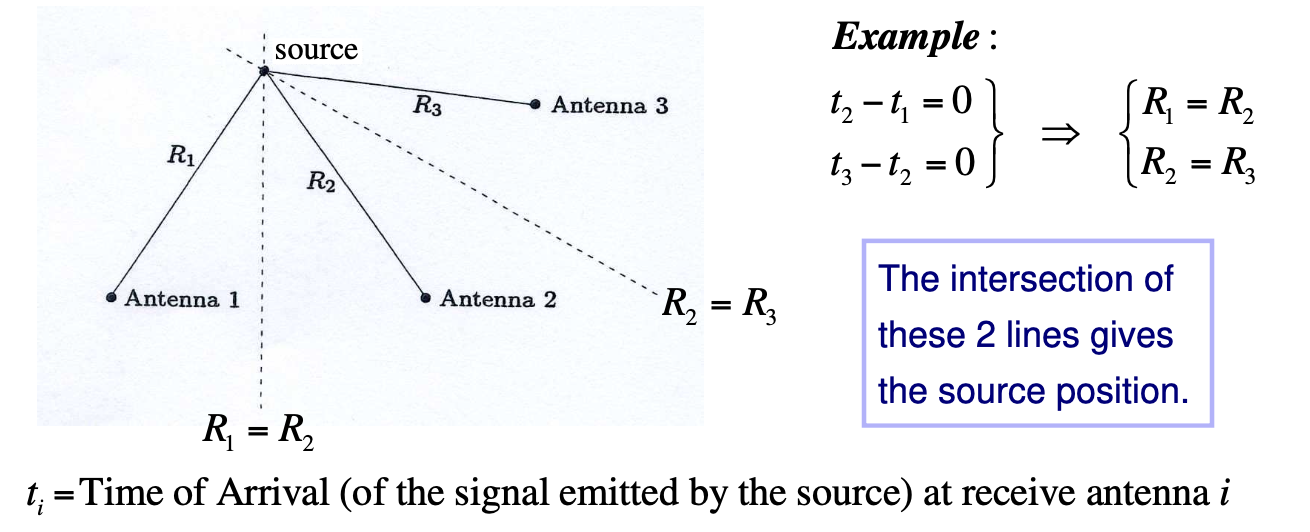
\includegraphics[width=0.75\linewidth]{Image/pdf 5/10.Source_localization.png}
        \label{fig:placeholder}
    \end{figure}
    \item The ToA \(t_i\) can be measured (i.e. estimated) as the location of the peak of the Matched Filter output or the Energy detector (ED).
    \item REMEMBER: in a more general situation for which the TDOAs are not zero the dashed lines become \textbf{hyperbolas}, the intersection again giving the source position.
    \item \underline{We need at least 3 receive sensors for localization}, and when the noise is present in the measurements, it is desirable to have more.
    \item Assume that \(N\) receive sensors (e.g. receive antennas) have been placed at known locations and that the \textbf{Time of Arrival (TOA)} measurements \(t_i\) for \(i=0,1,2,\cdots,N-1\) are available and assume that the source and the recieve sensors are on the same plane (2D problem).
    \item The problem is to estimate the source position \((x_s,y_s)\) from the observation of the \(N\) arrival times \(\{t_i=0,1,\cdots,N-1\}\).
\begin{figure}[H]
    \centering
    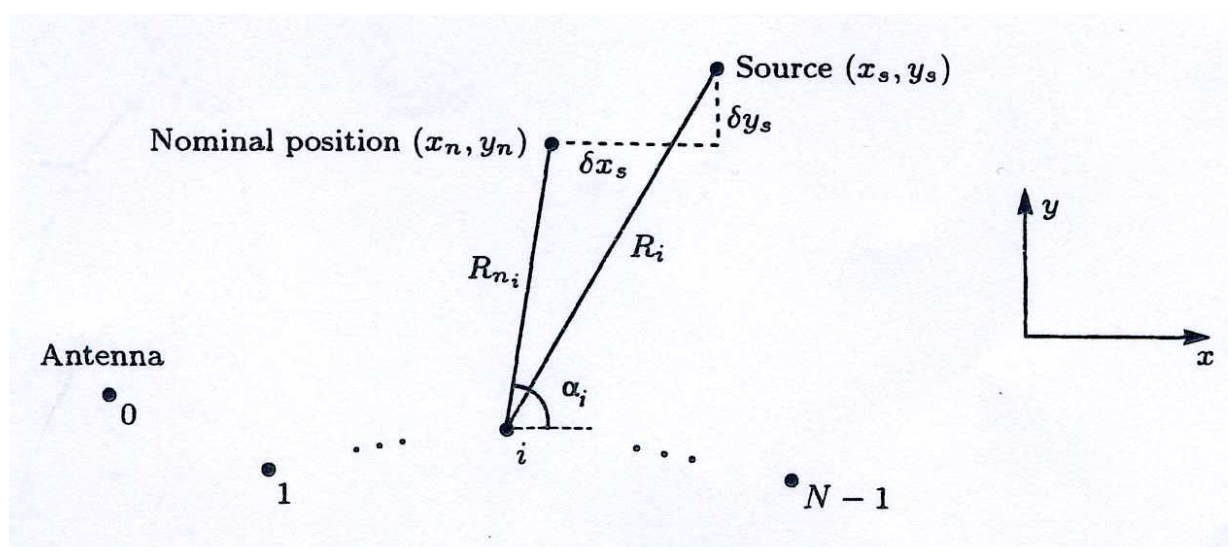
\includegraphics[width=0.75\linewidth]{Image/pdf 5/11.Source_loc_2.png}
    \label{fig:placeholder}
\end{figure}
    \item The (measured) times of arrival \(\{t_i\}\) are assumed to be corrupted by noise with zero mean and known covariance but otherwise unknown distribution.
    \item For a signal emitted by the source at time \(t=T_0\), the ToA measuerements are modeled by:
    \[
    t_i=T_0+\frac{R_i}{c}+e_i \qquad i=0,1,2,\cdots,N-1 
    \]
    \item When \(e_i\) are the measurements noises and \(c\) denotes the propagation speed.
    \item The noise samples are assumed to be zero mean with variance \(\sigma^2\) and uncorrelated with each other. \underline{No assumptions are made about the pdf of the noise}.
    \item Knowledge of \(T_0\) would require accurate clock synchronization between the source and the receivers. Often for economic reasons this is avoided. \underline{We assume here that the time \(T_0\) when the}\\ \underline{ source emits a signal is unknown}.

    \item Unknown position vector: \(\boldsymbol{\theta}=[x_s \quad y_s]^T\)
    \item Position of the \(i\)-th receiver sensor: \(\textbf{p}_i=[x_i\qquad y_i]^T\)
    \item Range between source and receive sensor \(i\)-th:
    \[
R_i = \lVert \boldsymbol{\theta} - \mathbf{p}_i \rVert
    = \sqrt{(x_s - x_i)^{2} + (y_s - y_i)^{2}},
    \qquad i = 0,1,2,\ldots,N-1
\]

    \item To remove the dependency of the observed data on the unknown time \(T_0\), it is customary to consider difference of arrivals or \underline{TDOA measurements}:
\begin{align*}
\tau_i
&= t_i - t_{i-1}
 = \frac{R_i - R_{i-1}}{c} + e_i - e_{i-1}
 = \frac{R_i - R_{i-1}}{c} + w_i,
 \qquad i = 1,2,\ldots,N-1 \\[6pt]
&= \frac{
\sqrt{(x_s - x_i)^{2} + (y_s - y_i)^{2}}
-
\sqrt{(x_s - x_{i-1})^{2} + (y_s - y_{i-1})^{2}}
}{c}
+ w_i
\end{align*}

    \item \textbf{TDOA data model}:
\[
\boldsymbol{\tau}_{(N-1)\times 1}
= \mathbf{s}(\boldsymbol{\theta}) + \mathbf{w},
\qquad
\boldsymbol{\theta} =
\begin{bmatrix}
x_s \\[2pt]
y_s
\end{bmatrix}
\]

\[
s_i(\boldsymbol{\theta})
= \frac{R_i - R_{i-1}}{c}
= \frac{
\sqrt{(x_s - x_i)^{2} + (y_s - y_i)^{2}}
-
\sqrt{(x_s - x_{i-1})^{2} + (y_s - y_{i-1})^{2}}
}{c}
\]

    \item To estimate the unknown parameter vector \(\theta\) we could use the \textbf{Non linear Least Squares (NLLS)} method:
    \[
    \hat{\boldsymbol{\theta}}_{NLLS} =\underset{\theta}{\arg\min}||\boldsymbol{\tau}-\mathbf{s}(\boldsymbol{\theta})||^2
    \]
    \item The NLLS estimator does not require statistical characterization of the noise vector \textbf{w}, but it is computationally heavy (it requires iterative optimization techniques).
    \item Let us now assuma that a \textbf{nominal source position} \((x_n,y_n)\) is available that is close to the true source position.
    \item Such a situation is typical when a source is being tracked; in that case the nominal position is the position of the source at the previous measurement time.
    \begin{figure}
        \centering
        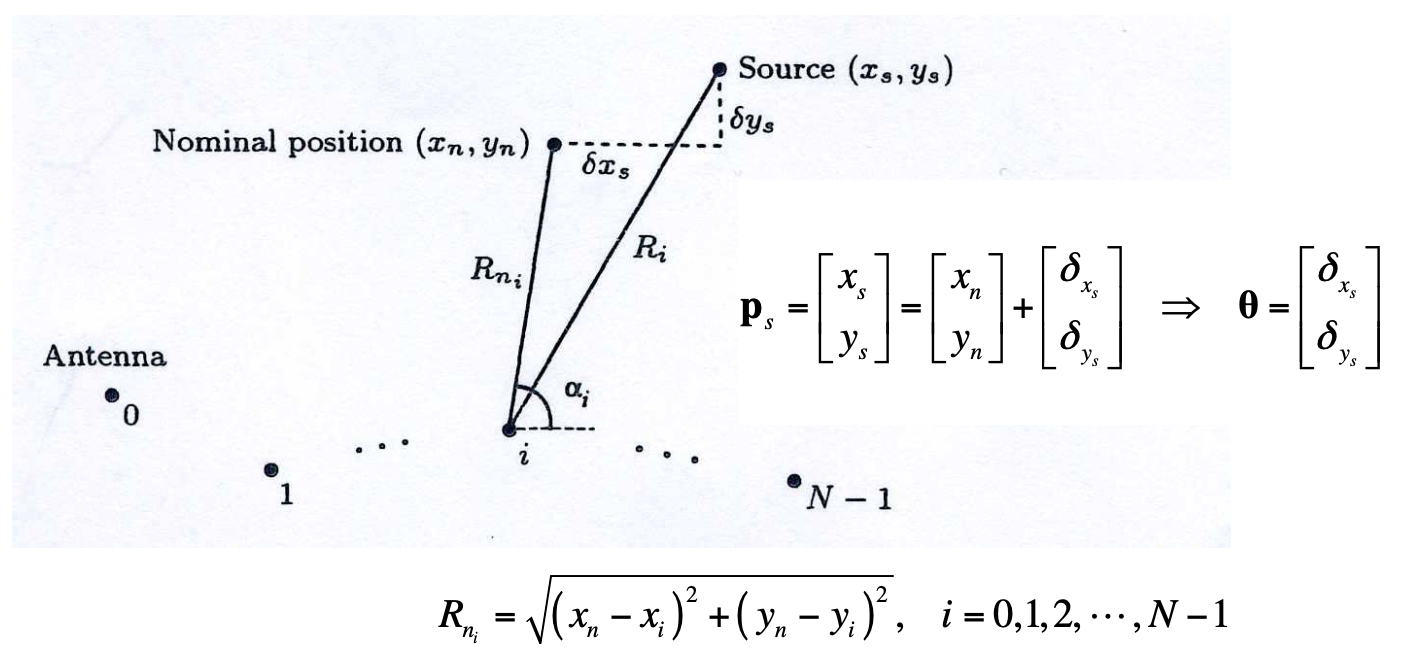
\includegraphics[width=0.75\linewidth]{Image/pdf 5/12.Source_loc-3.png}
        \label{fig:placeholder}
    \end{figure}
    \item Range between source and receive sensor \(i\)-th as a function of the nominal position:
    \[
R_i
= \sqrt{(x_s - x_i)^{2} + (y_s - y_i)^{2}}
= \sqrt{(x_n + \delta_{x_s} - x_i)^{2}
       + (y_n + \delta_{y_s} - y_i)^{2}}
\]
    \item If we now use a first-order Taylor expansio of \(R_i\), considered as a 2D function of the source position \((x_s,y_s)\) about the nominal position (\((x_n,y_n)\)) we get:
\begin{align*}
R_i
&\approx R_{n_i}
 + \frac{x_n - x_i}{R_{n_i}}\,\delta_{x_s}
 + \frac{y_n - y_i}{R_{n_i}}\,\delta_{y_s}  = R_{n_i}
 + \cos(\alpha_i)\,\delta_{x_s}
 + \sin(\alpha_i)\,\delta_{y_s}
\end{align*}
\begin{align*}
\tau_i
&= \frac{R_i - R_{i-1}}{c} + w_i\approx \frac{R_{n_i} - R_{n_{i-1}}}{c}
 + \frac{\cos(\alpha_i) - \cos(\alpha_{i-1})}{c}\,\delta_{x_s}
 + \frac{\sin(\alpha_i) - \sin(\alpha_{i-1})}{c}\,\delta_{y_s}
 + w_i
\end{align*}

    \item \textbf{\underline{Linearized} measurement data model}:
    \[
z_i
= \tau_i - \frac{R_{n_i} - R_{n_{i-1}}}{c}
= \frac{\cos\alpha_i - \cos\alpha_{i-1}}{c}\,\delta_{x_s}
 + \frac{\sin\alpha_i - \sin\alpha_{i-1}}{c}\,\delta_{y_s}
 + w_i
\]
\[
\mathbf{z}_{(N-1)\times 1} = \mathbf{H}\boldsymbol{\theta} + \mathbf{w},
\qquad
\boldsymbol{\theta} =
\begin{bmatrix}
\delta_{x_s} \\[2pt]
\delta_{y_s}
\end{bmatrix},
\qquad
\mathbf{w} =
\begin{bmatrix}
w_1 \\ \vdots \\ w_{N-1}
\end{bmatrix}
=
\begin{bmatrix}
e_1 - e_0 \\ \vdots \\ e_{N-1} - e_{N-2}
\end{bmatrix}
\]

\[
\mathbf{H}_{(N-1)\times 2}
= \frac{1}{c}
\begin{bmatrix}
\cos\alpha_1 - \cos\alpha_0 & \sin\alpha_1 - \sin\alpha_0 \\
\cos\alpha_2 - \cos\alpha_1 & \sin\alpha_2 - \sin\alpha_1 \\
\vdots & \vdots \\
\cos\alpha_{N-1} - \cos\alpha_{N-2} &
\sin\alpha_{N-1} - \sin\alpha_{N-2}
\end{bmatrix}
\]

\item The noise vector \textbf{w} is zero mean, correlated, with unknown distribution:

\item The covariance matrix of the noise vector \textbf{w} can be expressed as a function of the covariance matrix of the noise vector \textbf{e} in the TOA measurements (that we assumed to be uncorrelated):
\begin{align*}
\mathbf{C}_w
&= E\{\mathbf{w}\mathbf{w}^{T}\}
 = E\{(\mathbf{A}\mathbf{e})(\mathbf{A}\mathbf{e})^{T}\}
 = E\{\mathbf{A}\mathbf{e}\mathbf{e}^{T}\mathbf{A}^{T}\} \\[4pt]
&= \mathbf{A}E\{\mathbf{e}\mathbf{e}^{T}\}\mathbf{A}^{T}
 = \mathbf{A}\mathbf{C}_e\mathbf{A}^{T}
 = \mathbf{A}(\sigma^{2}\mathbf{I})\mathbf{A}^{T}
 = \sigma^{2}\mathbf{A}\mathbf{A}^{T}
\end{align*}

\item Thanks to the linearization, the problem has been recast as the problem of estimating the vector \(\theta\) based on th observation of the \((N-1)\)-dimensional vector \textbf{z}, when \textbf{H} is a-priori known and \textbf{w} is zero mean, correlated, with known covariance matrix \(\mathbf{C}_\text{w}\):
\[
\mathbf{z}_{(N-1)\times 1}
= \mathbf{H}\boldsymbol{\theta} + \mathbf{w},
\qquad
\boldsymbol{\theta} =
\begin{bmatrix}
\delta_{x_s} \\[2pt]
\delta_{y_s}
\end{bmatrix}
\]

\[
\mathbf{H}_{(N-1)\times 2}
= \frac{1}{c}
\begin{bmatrix}
\cos\alpha_1 - \cos\alpha_0 & \sin\alpha_1 - \sin\alpha_0 \\
\cos\alpha_2 - \cos\alpha_1 & \sin\alpha_2 - \sin\alpha_1 \\
\vdots & \vdots \\
\cos\alpha_{N-1} - \cos\alpha_{N-2} &
\sin\alpha_{N-1} - \sin\alpha_{N-2}
\end{bmatrix}
\]

\item Since we do not know the pdf of \textbf{w} we cannot derive the ML estimator. We can use the BLUE, which coincides with the WLS with weighting matrix equal to the inverse of the noise covariance matrix.
\item \textbf{BLUE/WLS estimator and MSE matrix}:
\begin{align*}
&\hat{\boldsymbol{\theta}}_{BLUE}
= \hat{\boldsymbol{\theta}}_{WLS}\Big|_{\mathbf{W}=\mathbf{C}_w^{-1}}
= (\mathbf{H}^{T}\mathbf{C}_w^{-1}\mathbf{H})^{-1}
  \mathbf{H}^{T}\mathbf{C}_w^{-1}\mathbf{z}
= \big(\mathbf{H}^{T}(\mathbf{A}\mathbf{A}^{T})^{-1}\mathbf{H}\big)^{-1}
  \mathbf{H}^{T}(\mathbf{A}\mathbf{A}^{T})^{-1}\mathbf{z}\\[4pt]
&E\{\hat{\boldsymbol{\theta}}_{BLUE}\} = \boldsymbol{\theta}\\[4pt]
&MSE\{\hat{\boldsymbol{\theta}}_{BLUE}\}
= (\mathbf{H}^{T}\mathbf{C}_w^{-1}\mathbf{H})^{-1}
= \sigma^{2}\big(\mathbf{H}^{T}(\mathbf{A}\mathbf{A}^{T})^{-1}\mathbf{H}\big)^{-1}
\end{align*}

\item If the noise vector is Gaussian distributed, this estimator is also the ML estimator and it is efficient.

\item \textbf{Example}: \(N=3\) elements Uniform Linear Array (ULA) line array (3 is the minimum number of antennas required):
\begin{figure}[H]
    \centering
    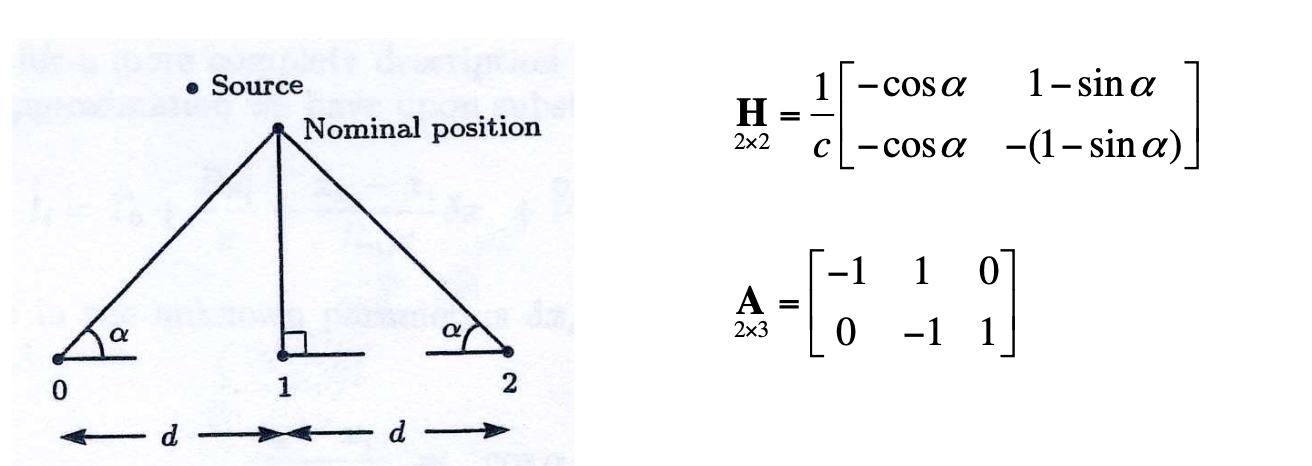
\includegraphics[width=0.75\linewidth]{Image/pdf 5/13.source_loc_4.png}
    \label{fig:placeholder}
\end{figure}
\(d\) is the so-called array \textbf{baseline}

\item For best localization we would like the angle to \(\alpha\) to be small. This is achieved by making the \textbf{baseline} \(d\) large the \textbf{array aperture}, i.e. the total length. Note also that the localization accuracy is range dependent, with the best accuracy for short ranges or for \(\alpha\) small.
(Dalla slide 93 ha salta)

\end{itemize}

\clearpage